\documentclass{beamer}
% Class options include: notes, handout, trans
%                        

% Theme for beamer presentation 
% Other themes include: beamerthemebars, beamerthemelined,beamerthemetree, beamerthemeplain
\usepackage{alltt}
\usepackage{underscore}
\usepackage[utf8]{inputenc}
\usepackage[activeacute,spanish]{babel}
\usepackage{verbatim}
\usepackage{graphicx}
\usepackage{amsmath}
\usepackage{amsfonts}
\usepackage{pdflscape}
\usepackage{inconsolata}
\usepackage{url}
\usepackage{listings}
\usepackage{soul}
\usepackage{listings}
\usepackage[section]{placeins}
\graphicspath{ {images/} }

\definecolor{listinggray}{gray}{0.9}
\definecolor{lbcolor}{rgb}{0.9,0.9,0.9}
\lstset{language=SQL, 
		basicstyle=\ttfamily\tiny, 
		showspaces=false, 
		numbers=left, 
		breaklines=true,
		frame=shadowbox
		}


\usefonttheme{professionalfonts}


\title[Seguridad Informática]{Seguridad Informática}
\subtitle{Proyecto 1}    % Enter your title between curly braces
\author[M. Jorquera, E. Regla, A. Valenzuela]{
	Miguel Jorquera, Erik Regla, Ariel Valenzuela\\
	\{mjorquera16,eregla09,arvalenzuela16\}\\@alumnos.utalca.cl}                 % Enter your name between curly braces
\institute[UTalca]{Universidad de Talca}      % Enter your institute name between curly braces
\date{\today}      % Enter the date or \today between curly braces



\defbeamertemplate{section page}{mine}[1][]{%
  \begin{centering}
    {\usebeamerfont{section name}\usebeamercolor[fg]{section name}#1}
    \vskip1em\par
    \begin{beamercolorbox}[sep=12pt,center]{part title}
      \usebeamerfont{section title}\insertsection\par
    \end{beamercolorbox}
  \end{centering}
}

\defbeamertemplate{subsection page}{mine}[1][]{%
  \begin{centering}
    {\usebeamerfont{subsection name}\usebeamercolor[fg]{subsection name}\insertsection~\insertsubsectionnumber}
    \vskip1em\par
    \begin{beamercolorbox}[sep=4pt,center]{part title}
      \usebeamerfont{subsection title}\insertsubsection\par
    \end{beamercolorbox}
  \end{centering}
}
\AtBeginSection{\frame{\sectionpage}}
\AtBeginSubsection{\frame{\subsectionpage}}

\setbeamertemplate{section page}[mine]
\setbeamertemplate{subsection page}[mine]

\begin{document}

% Creates title page of slide show using above information
\begin{frame}
  \titlepage
\end{frame}
\note{Talk for 30 minutes} % Add notes to yourself that will be displayed when typeset with the notes class option.

% Creates table of contents slide incorporating all \section and \subsection commands.
% \begin{frame}
%   \tableofcontents
% \end{frame}


\section{Introducción}
\begin{frame}[c,fragile]
	\frametitle{Introducción}

	En este documento se realizará la ejecución de un análisis de riesgos para un municipio ficticio.
	
	% , el cual cuenta con una serie de problemas administrativos derivados de previas administraciones y direcciones del departamento de tecnologías de la información.\\
	% Como referencia se usó la información real de municipios Chilenos, informes de contraloría y descripciones de procesos ya existentes en in intento de fidelizar el informe a la realidad diaria exagerando algunos atributos.
\end{frame}


\section{Introducción}
\begin{frame}[c,fragile]
	\frametitle{Introducción - Consideraciones}

	\begin{itemize}
		\item Se utilizó información de administraciones reales previas de municipios chilenos.
		\item Principalmente la información viene de informes emitidos de la Contraloría General de la República.
	\end{itemize}

	\\ \pause

	Muchas cosas podrán de ahora en adelante sonar alarmistas, sin embargo, la realidad es mucho peor de lo que está acá.
\end{frame}


\subsection{Estructura Organizacional}
\begin{frame}[c,fragile]
	\frametitle{Estructura Organizacional}


	\begin{figure}[H]
		\centering
		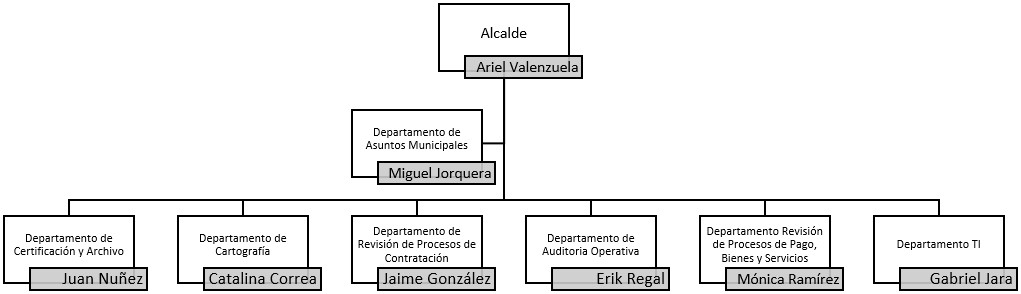
\includegraphics[width=1\textwidth]{../fragments/01structure/organigramaMunicipalidad.jpg}\\
	\caption{Organigrama}
	\label{FIG:ORGANIGRAMA}
	\end{figure}
	
\end{frame}

\begin{frame}[c,fragile]
	\frametitle{Departamentos a observar}
	\begin{itemize}
		\item{Departamento de Asuntos Municipales}
		\item{Departamento de Certificación y archivo}
		\item{Departamento de Cartografía }
		\item{Departamento de Revisión de Procesos de Contratación }
		\item{Departamento de Auditoría Operativa}
		\item{Dirección de revisión de Procesos de Pago, Bienes y Servicios}
		\item{Departamento de Tecnologías de la Información}
		\item{Alcaldía}
	\end{itemize}
\end{frame}


\begin{frame}[c,fragile]
	\frametitle{Sistemas externalizados}
	\begin{itemize}
		\item{Sistema de contabilidad gubernamental}
		\item{Sistema de tesorería municipal}
		\item{Sistema de patentes comerciales}
		\item{Sistema de permisos de circulación}
	\end{itemize}
\end{frame}

\begin{frame}[c,fragile]
	\frametitle{Sistemas externalizados - Versión simple}
	\begin{figure}[H]
		\centering
		
\includegraphics[width=.7\textwidth]{./images/1.png}\\
	\end{figure}
\end{frame}
\begin{frame}[c,fragile]
	\frametitle{Sistemas externalizados - Versión simple}
	\begin{figure}[H]
		\centering
		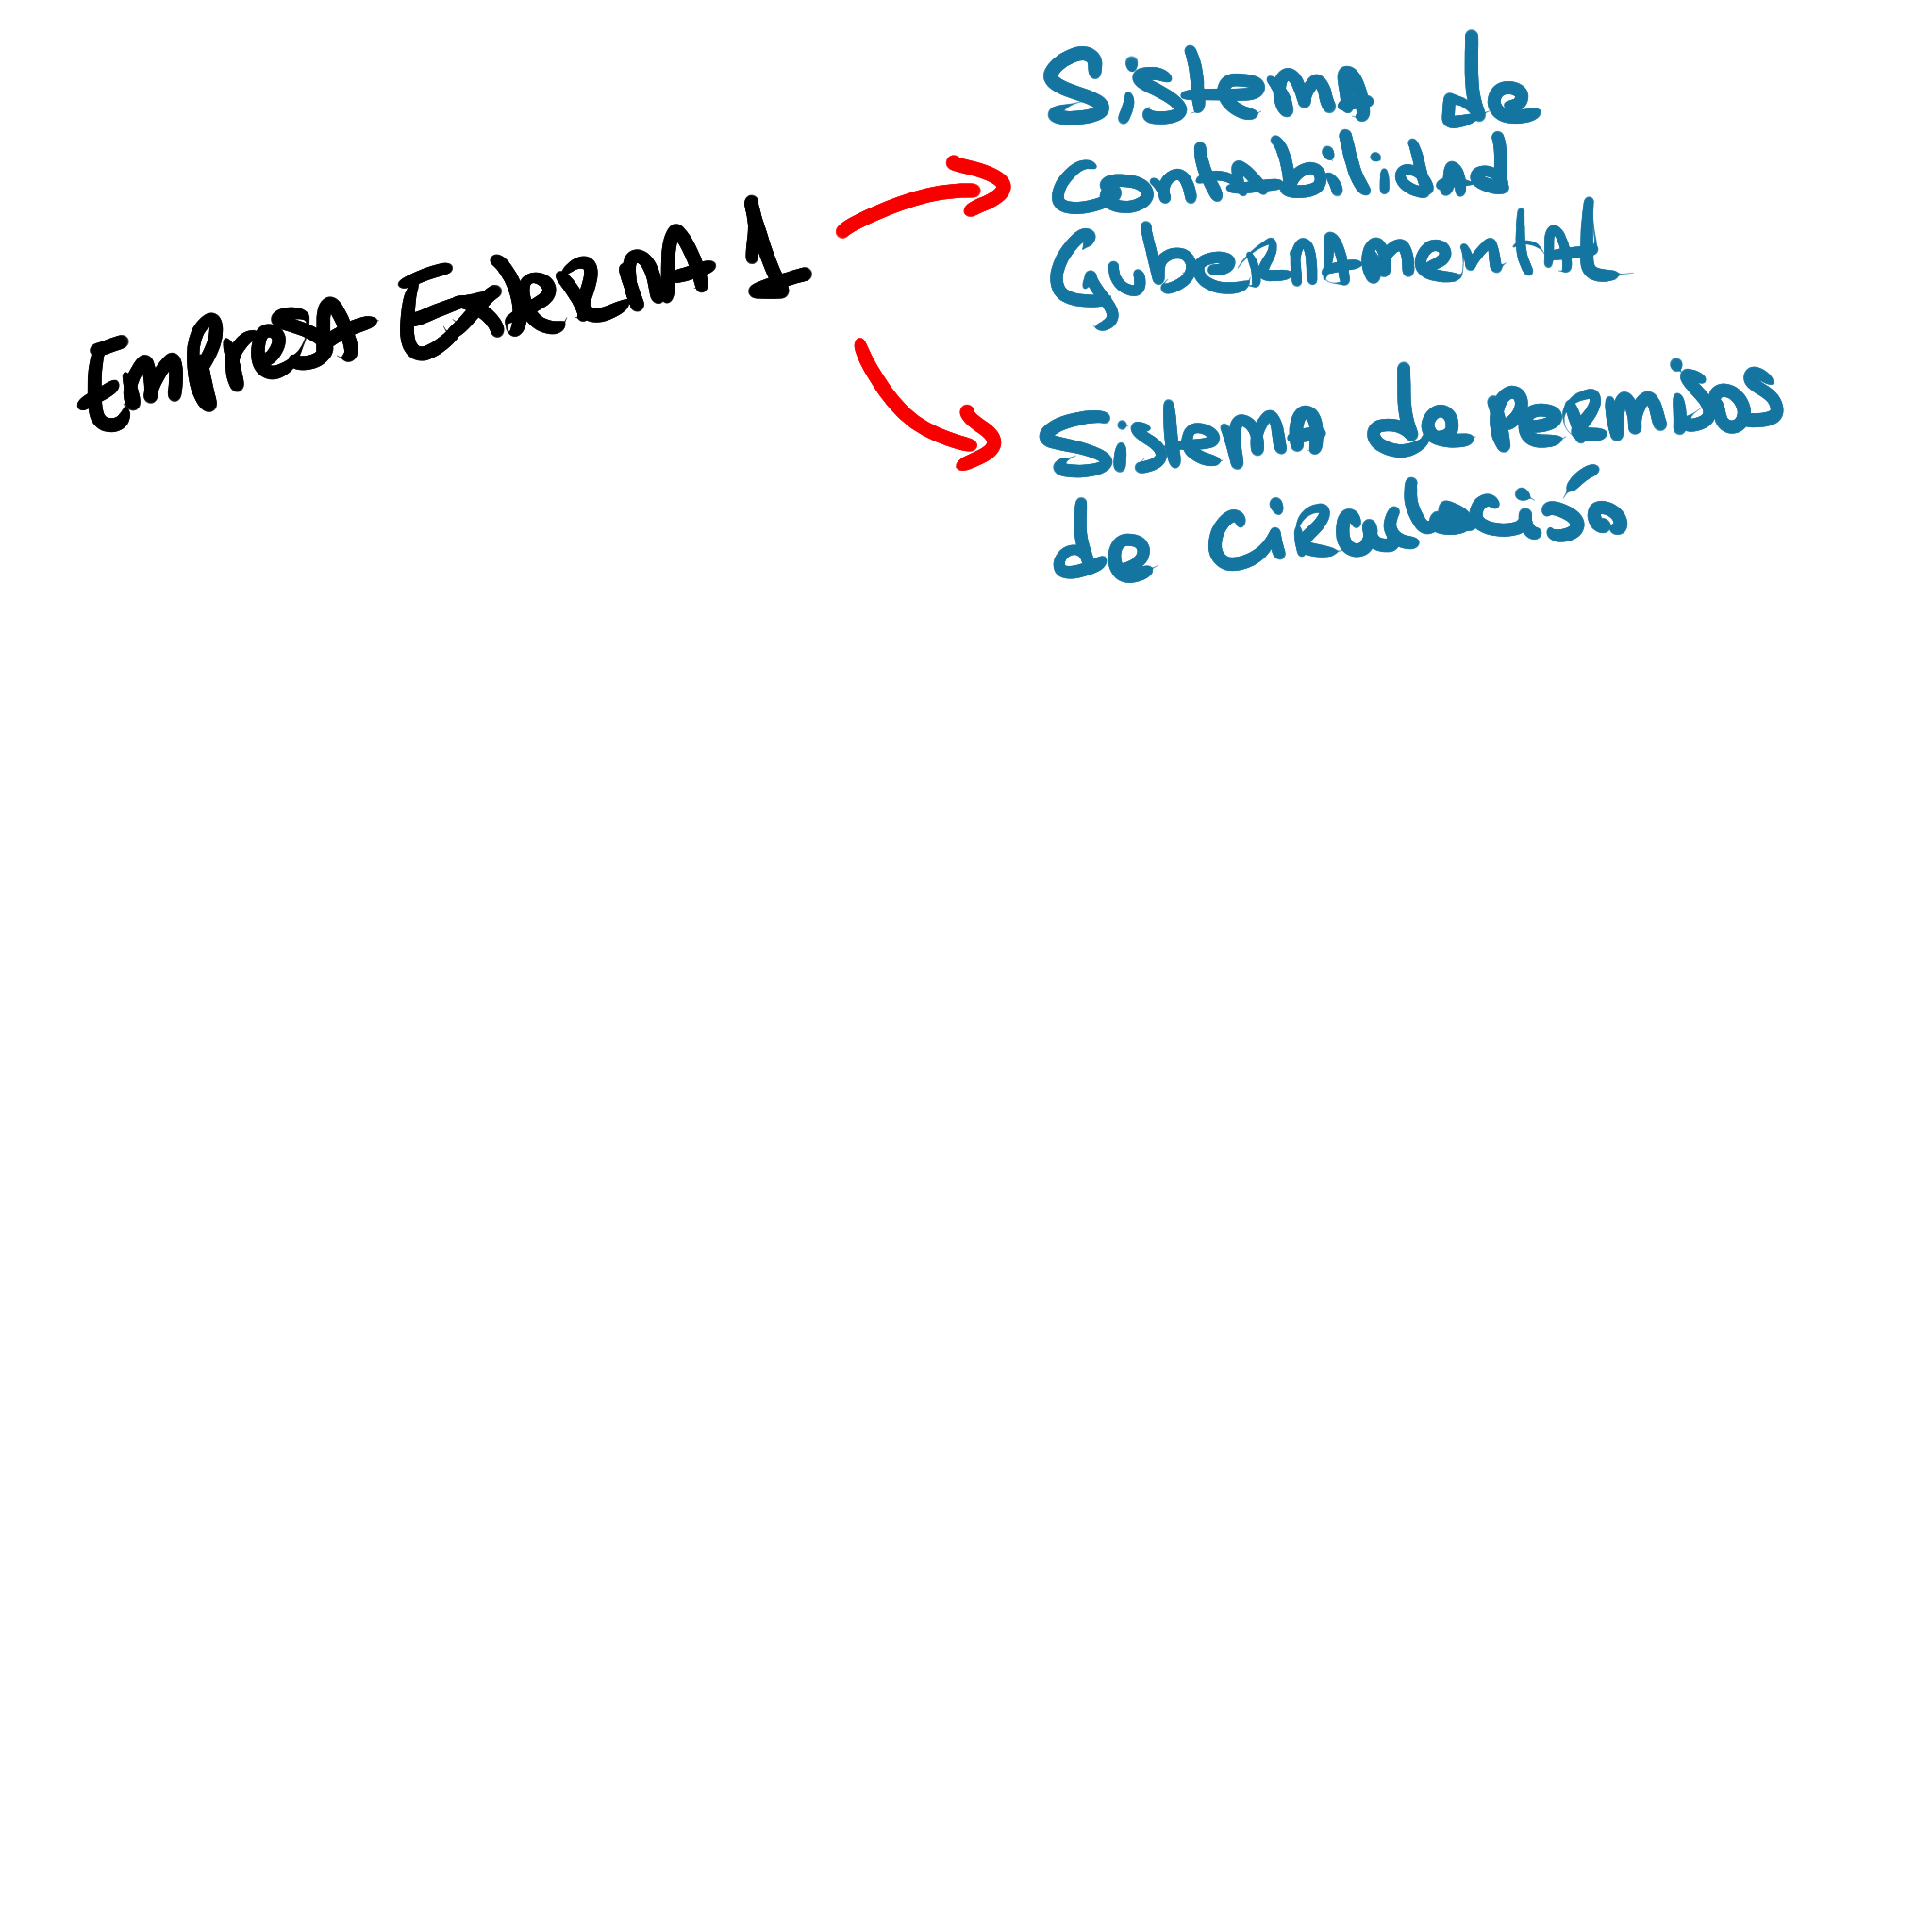
\includegraphics[width=.7\textwidth]{./images/2.png}\\
	\end{figure}
\end{frame}
\begin{frame}[c,fragile]
	\frametitle{Sistemas externalizados - Versión simple}
	\begin{figure}[H]
		\centering
		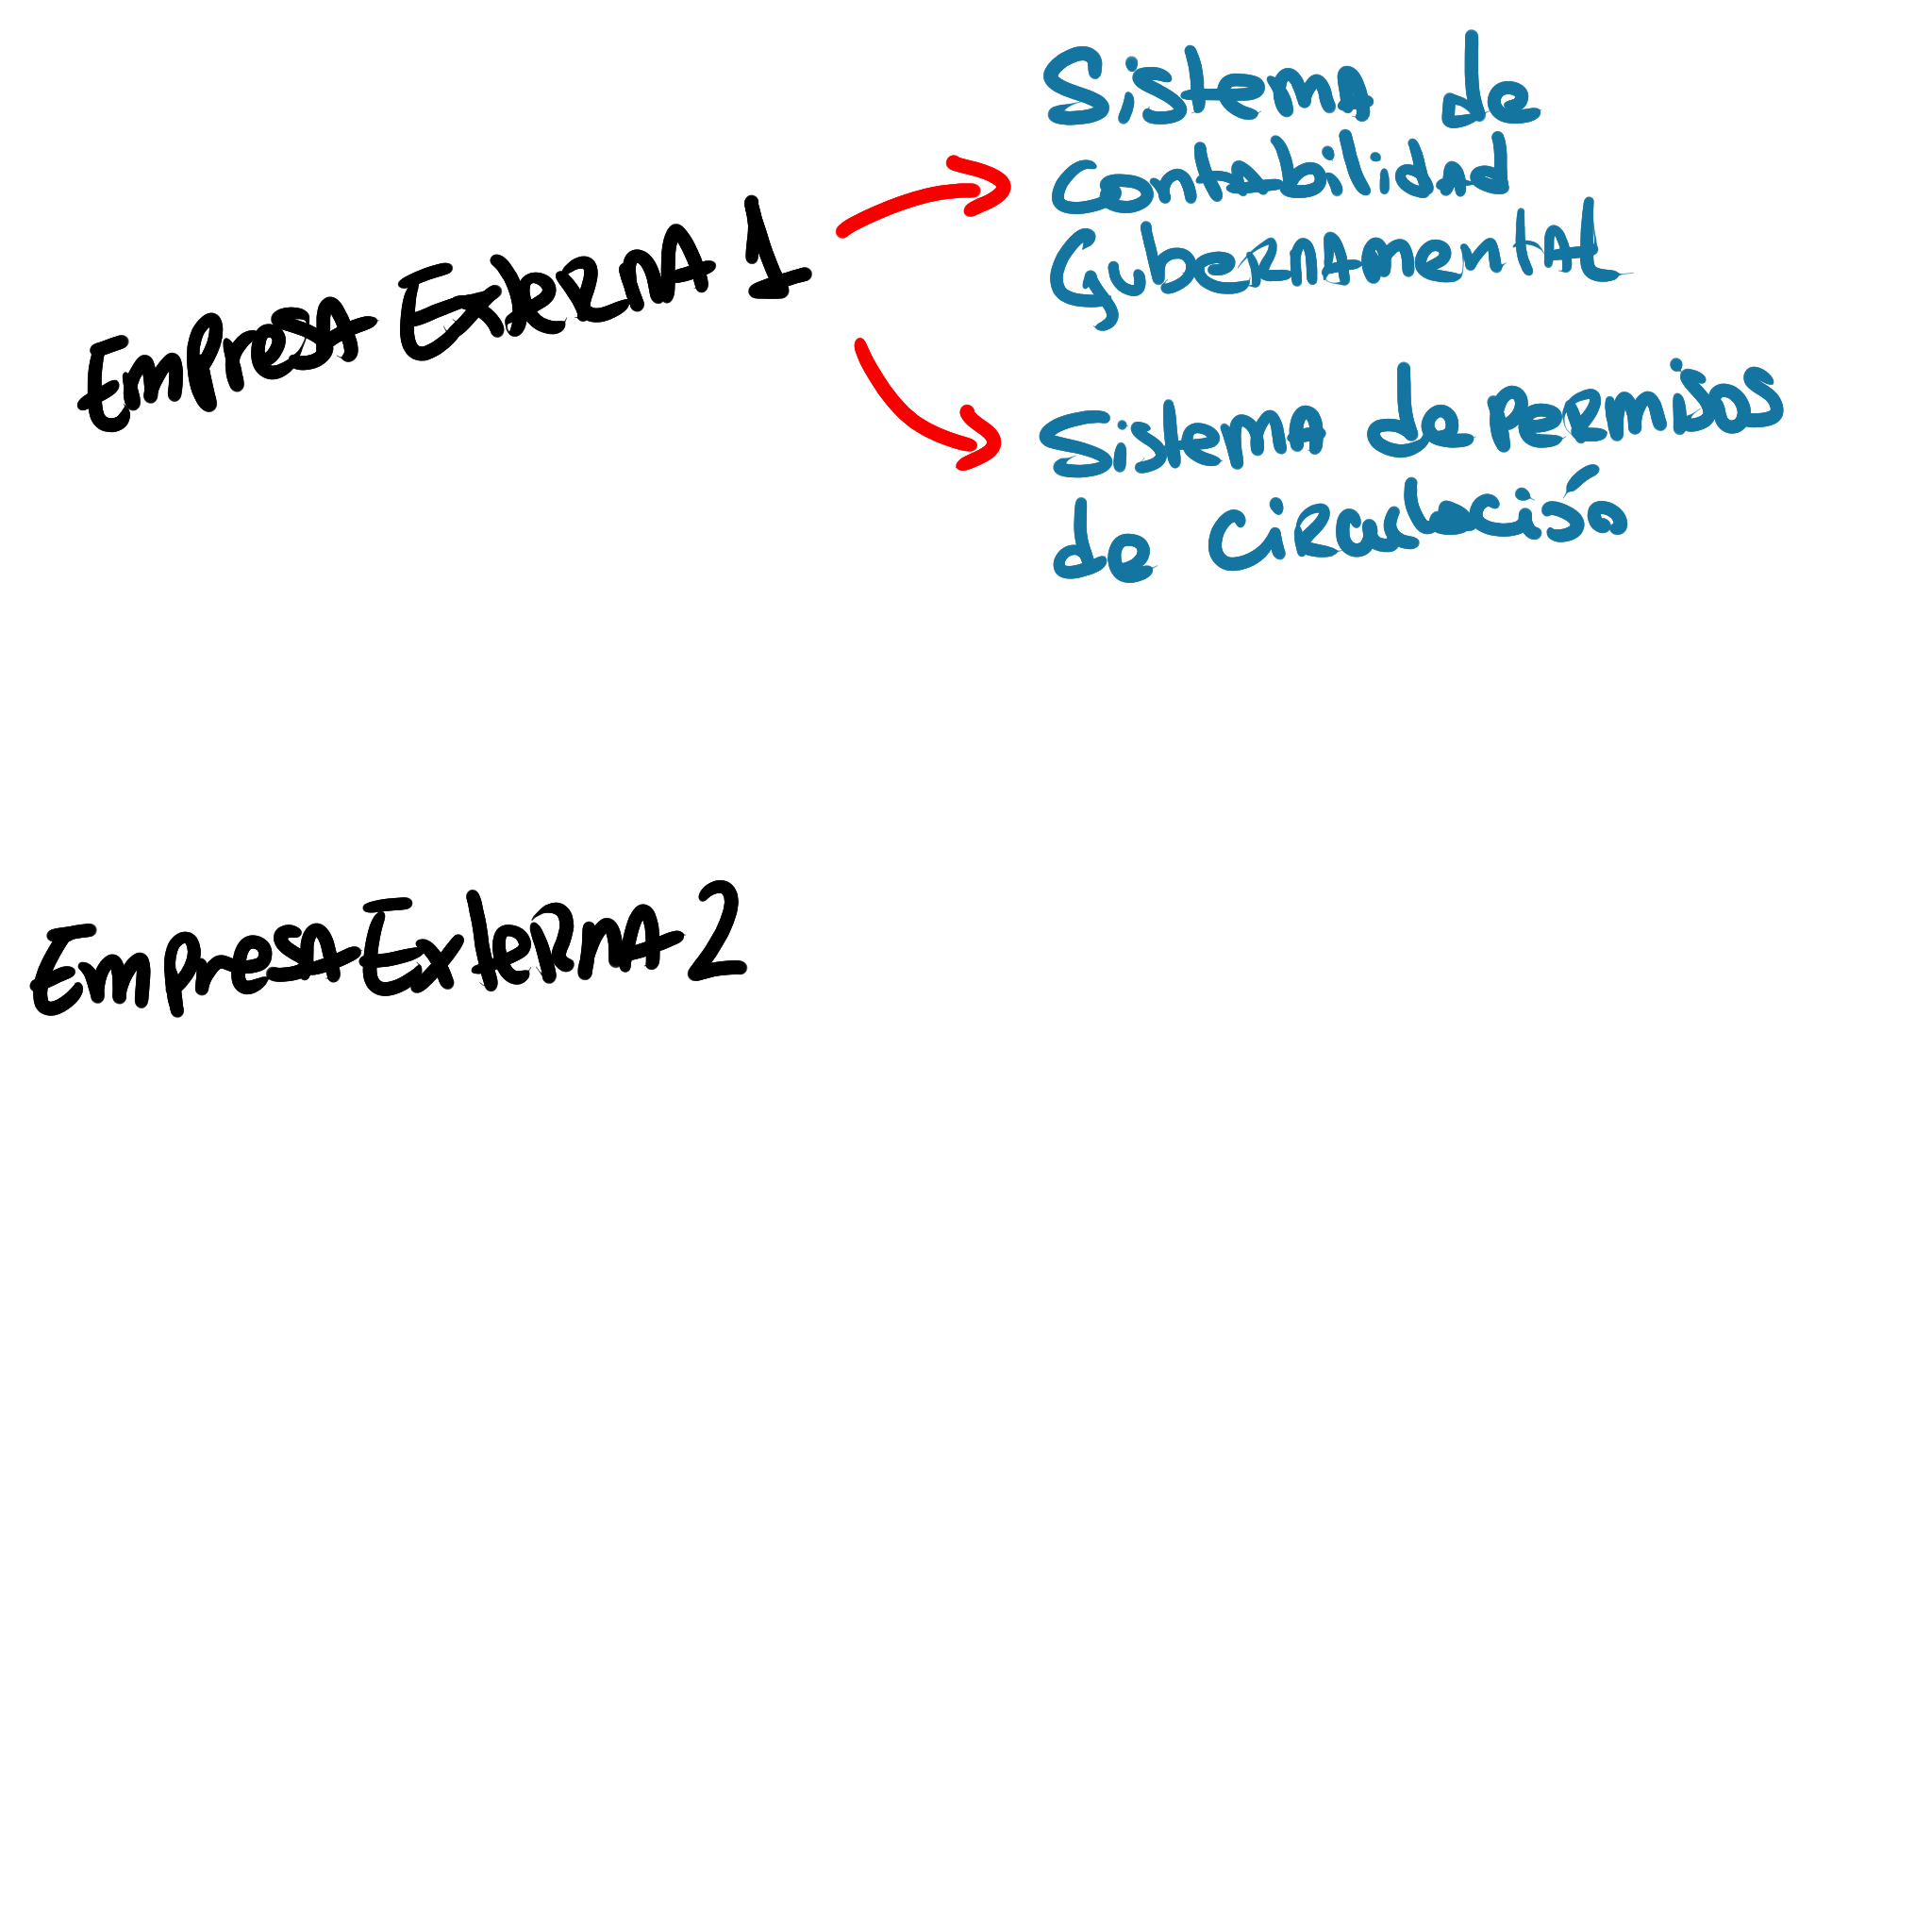
\includegraphics[width=.7\textwidth]{./images/3.png}\\
	\end{figure}
\end{frame}
\begin{frame}[c,fragile]
	\frametitle{Sistemas externalizados - Versión simple}
	\begin{figure}[H]
		\centering
		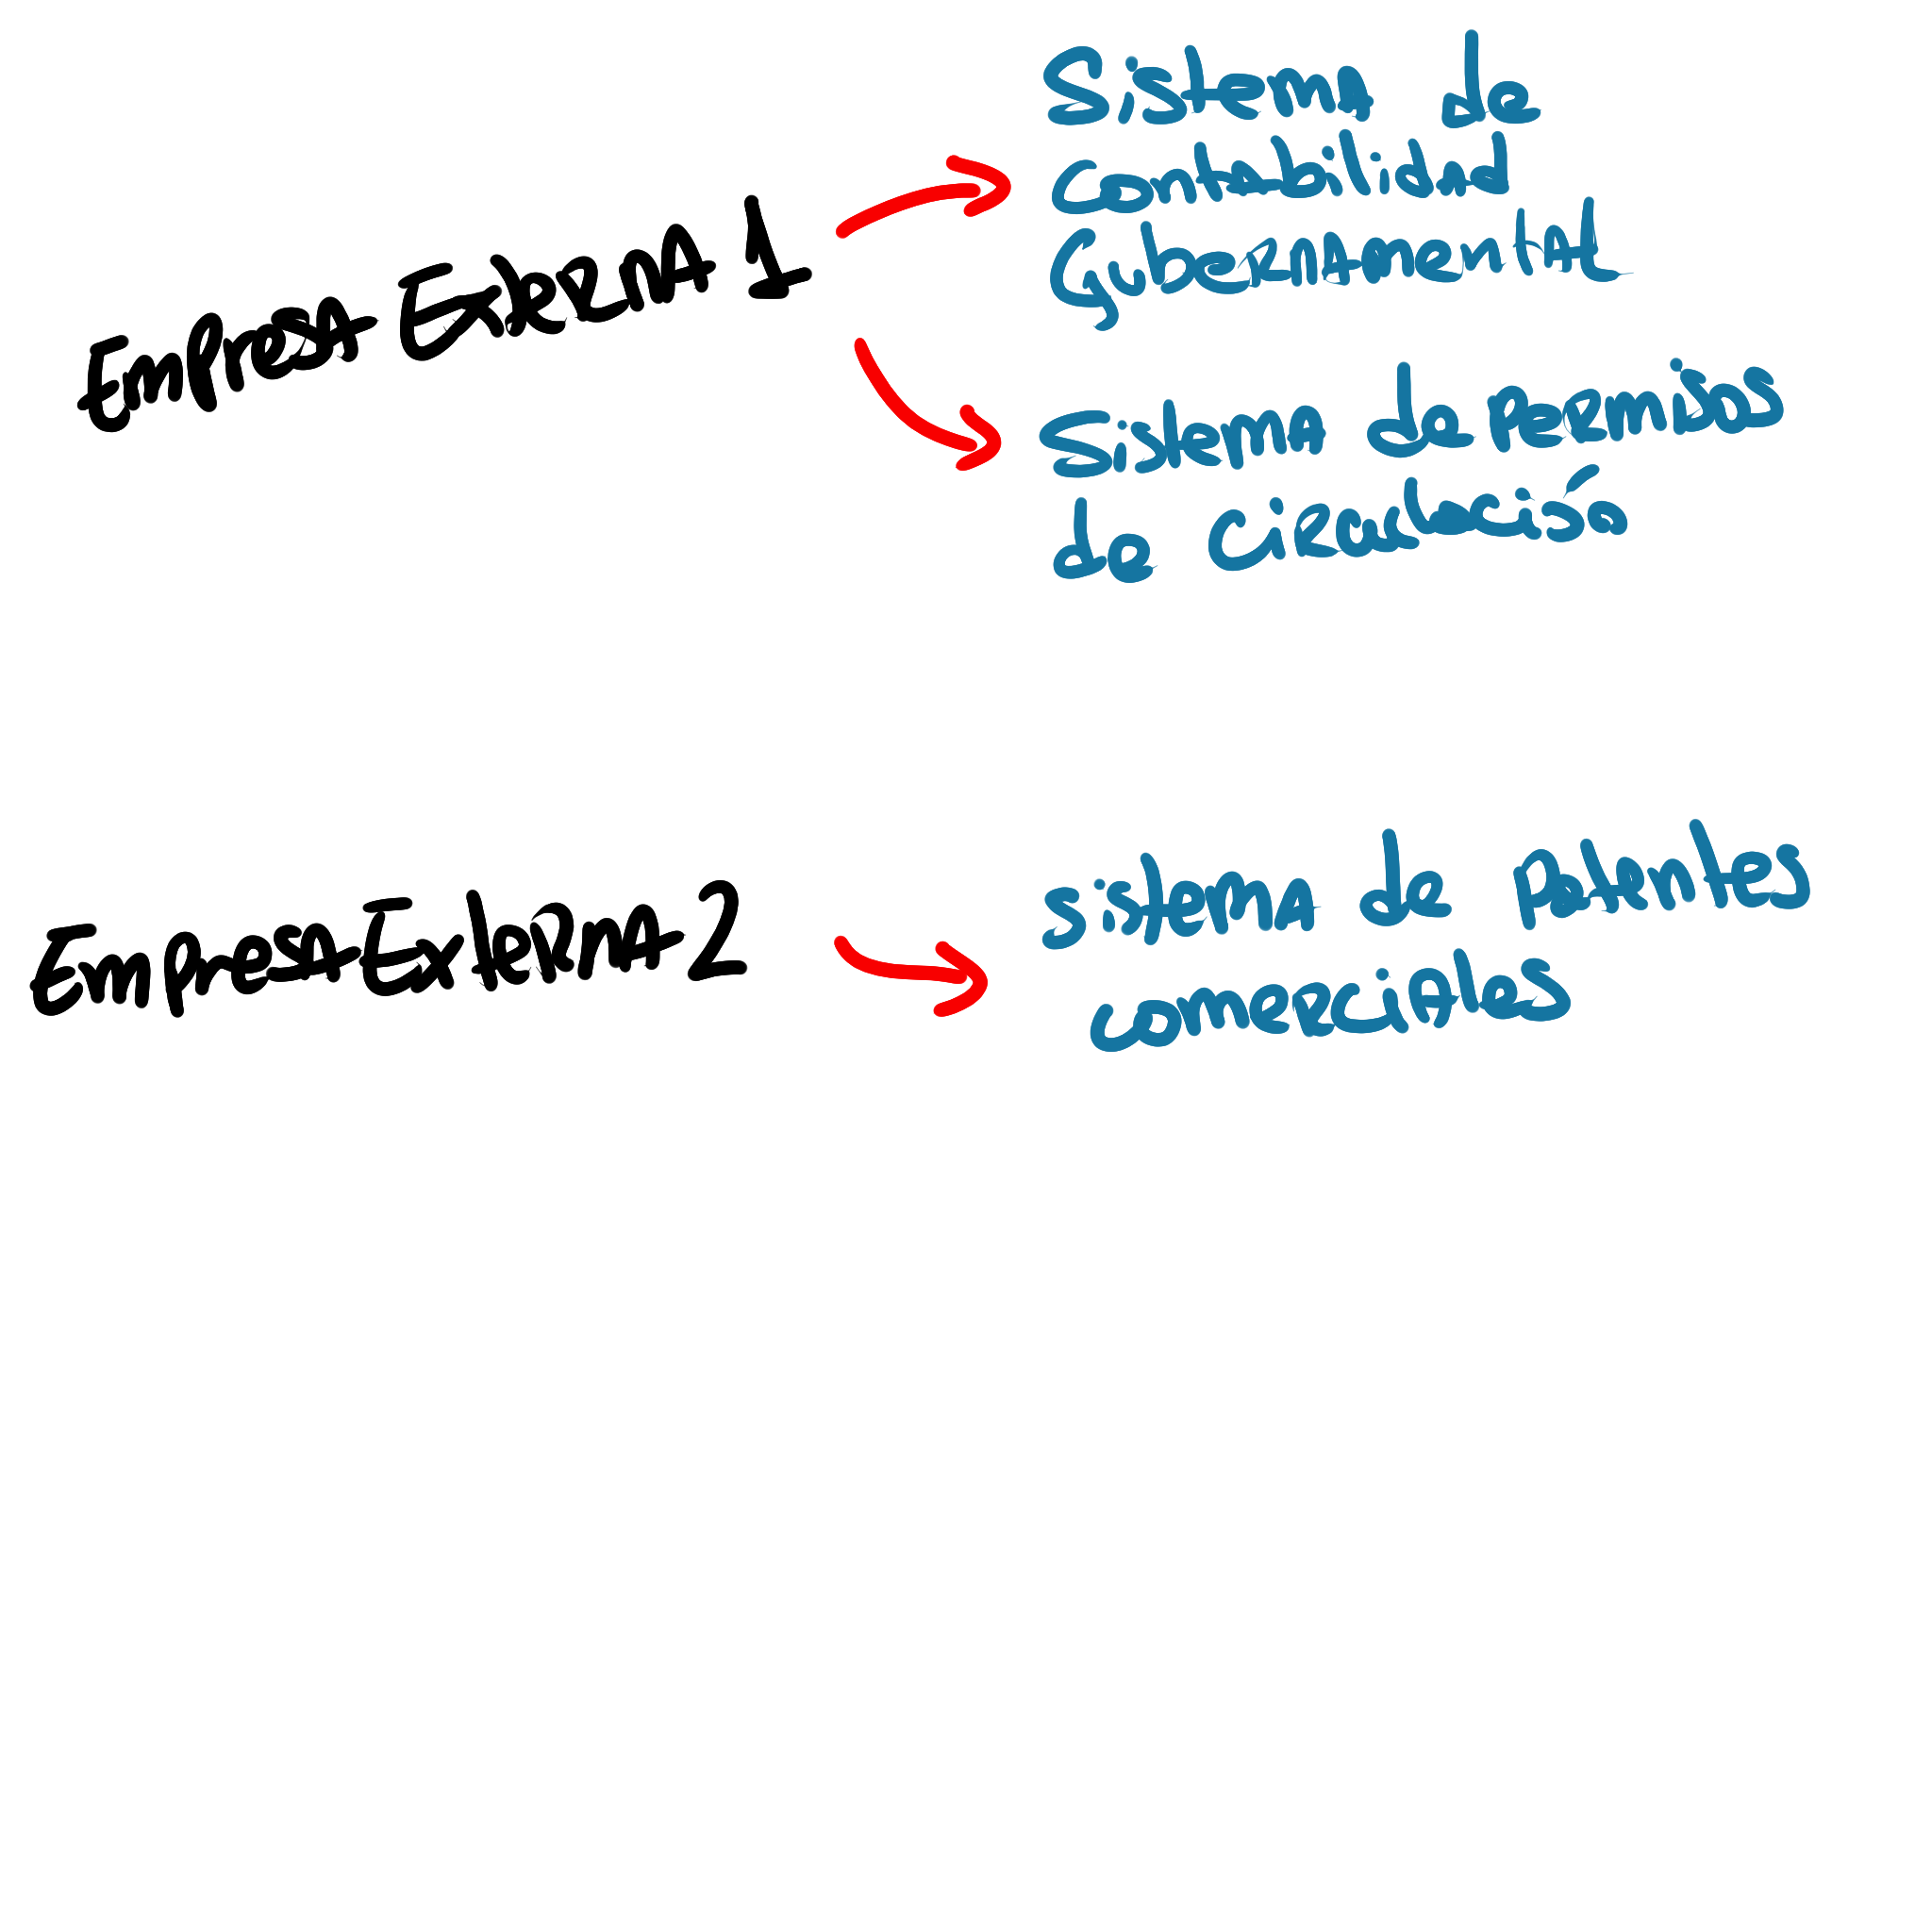
\includegraphics[width=.7\textwidth]{./images/4.png}\\
	\end{figure}
\end{frame}
\begin{frame}[c,fragile]
	\frametitle{Sistemas externalizados - Versión simple}
	\begin{figure}[H]
		\centering
		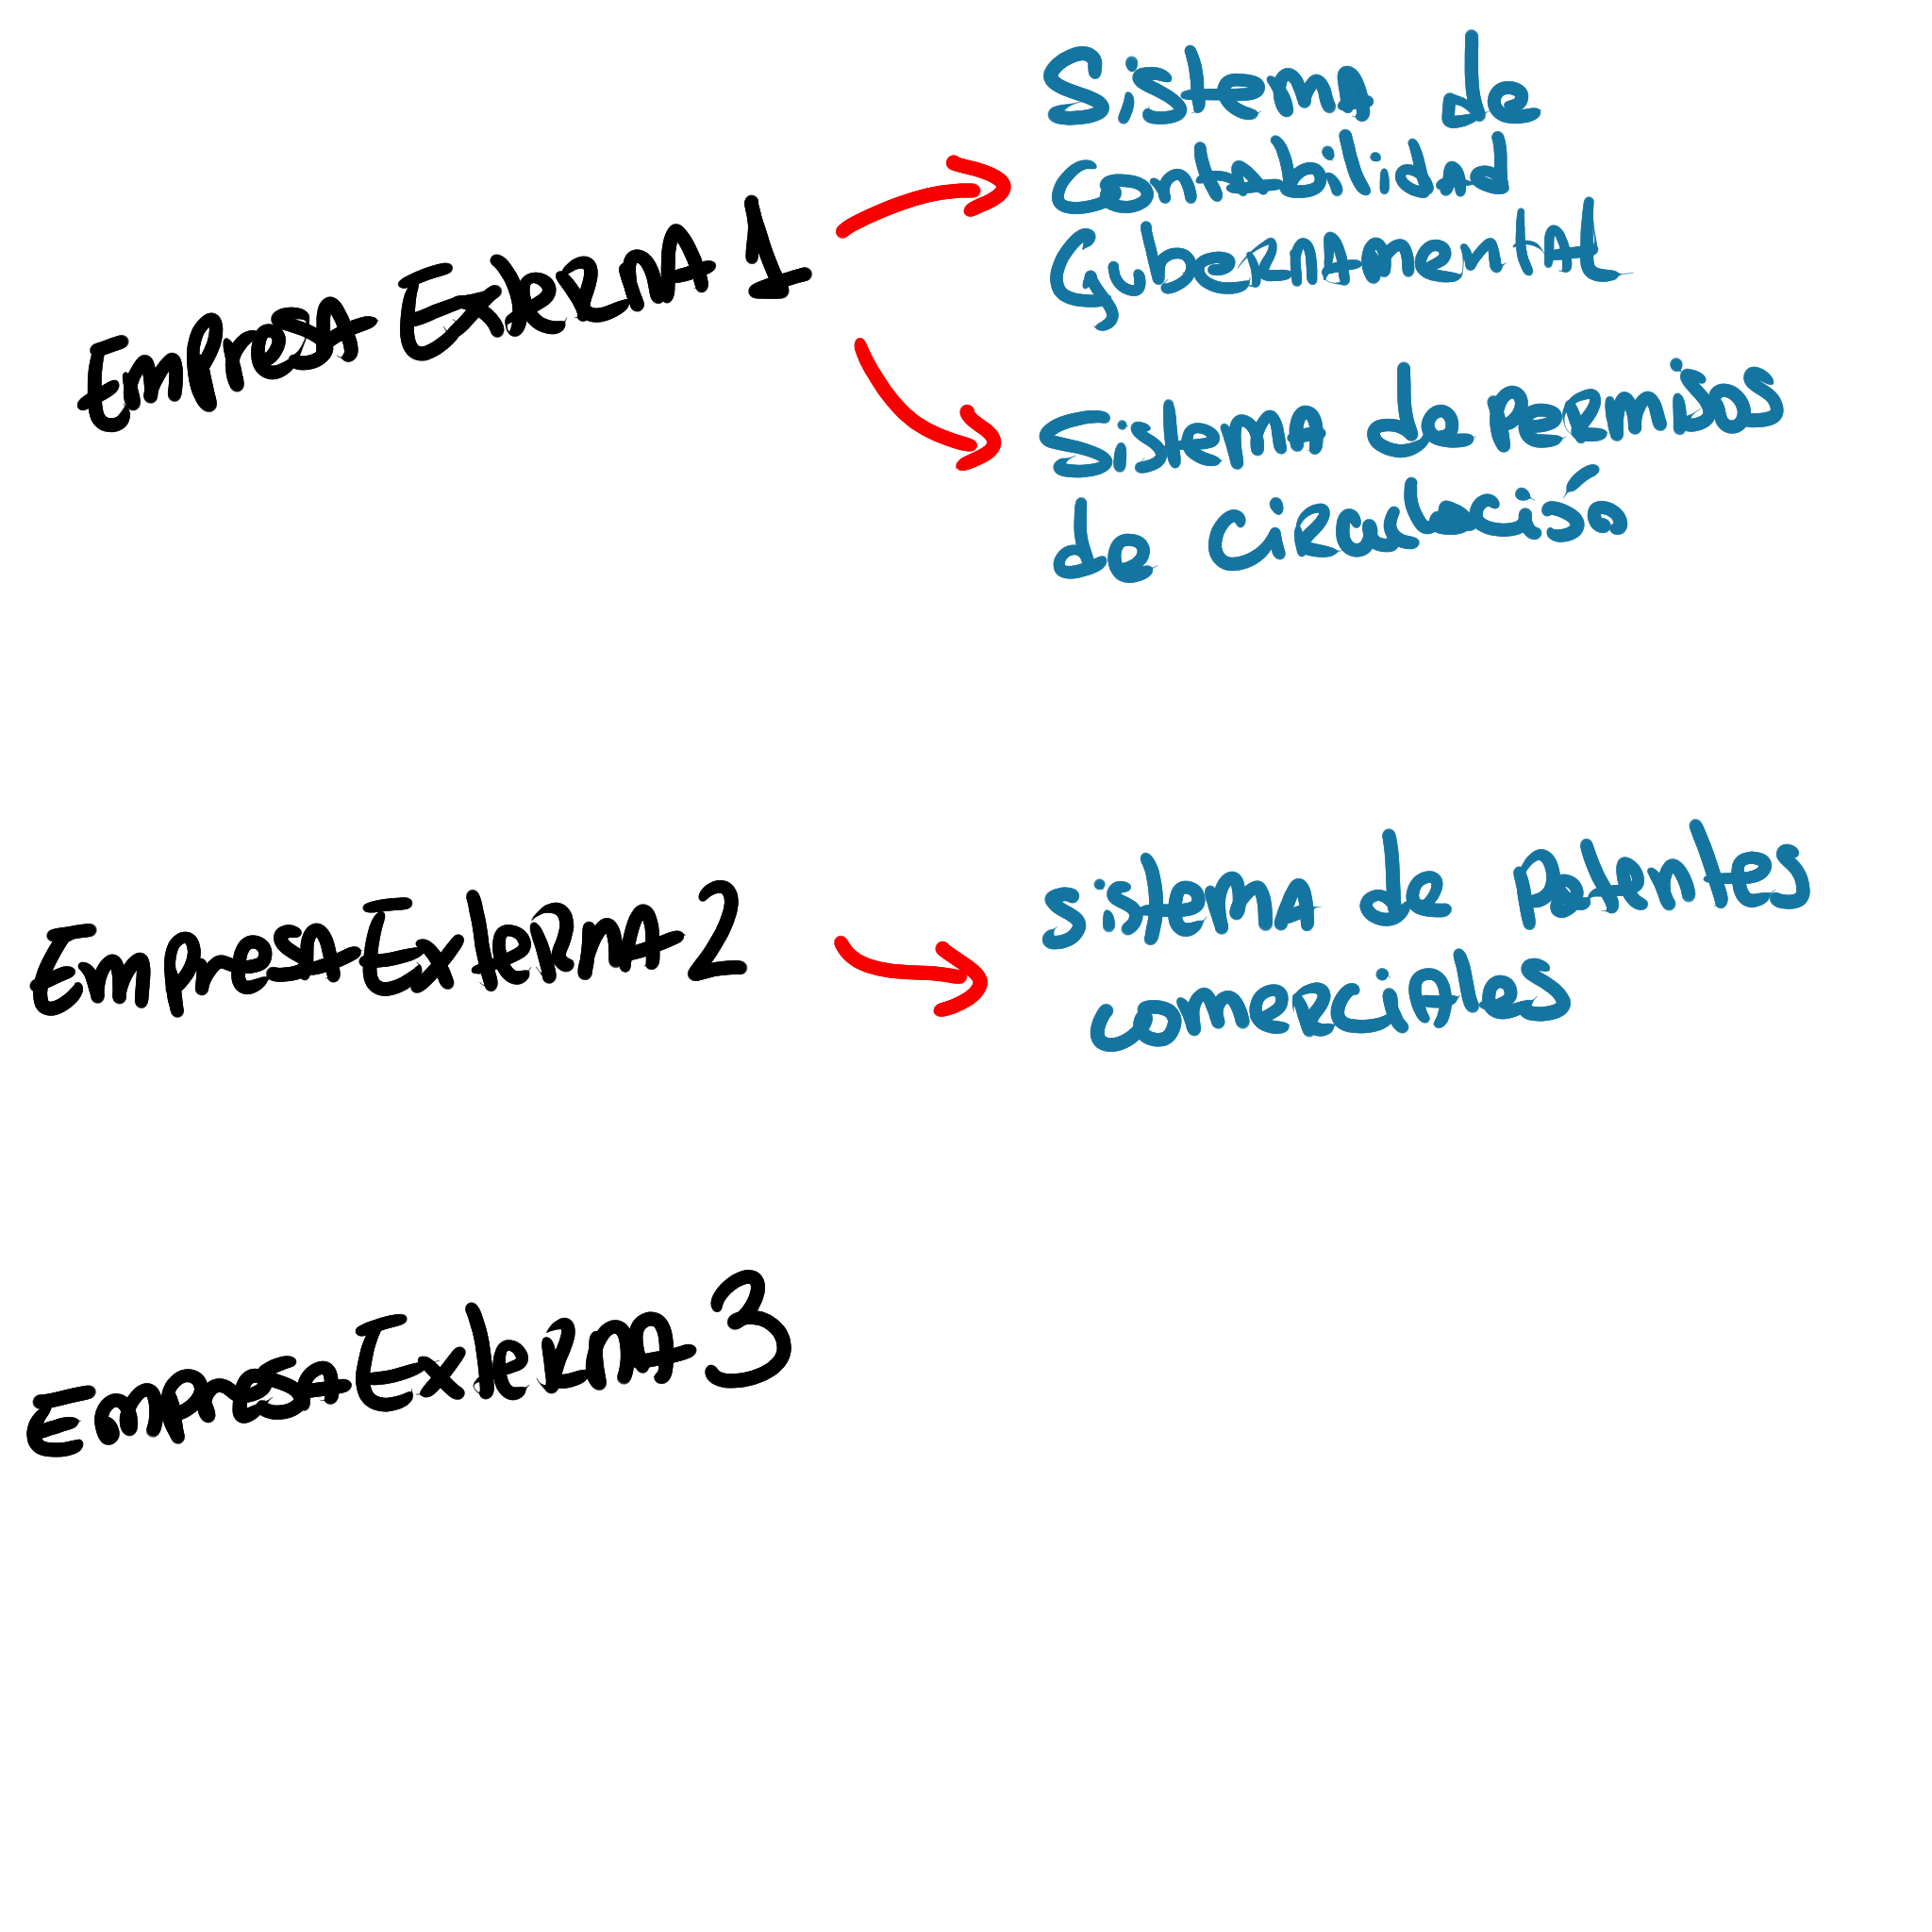
\includegraphics[width=.7\textwidth]{./images/5.png}\\
	\end{figure}
\end{frame}
\begin{frame}[c,fragile]
	\frametitle{Sistemas externalizados - Versión simple}
	\begin{figure}[H]
		\centering
		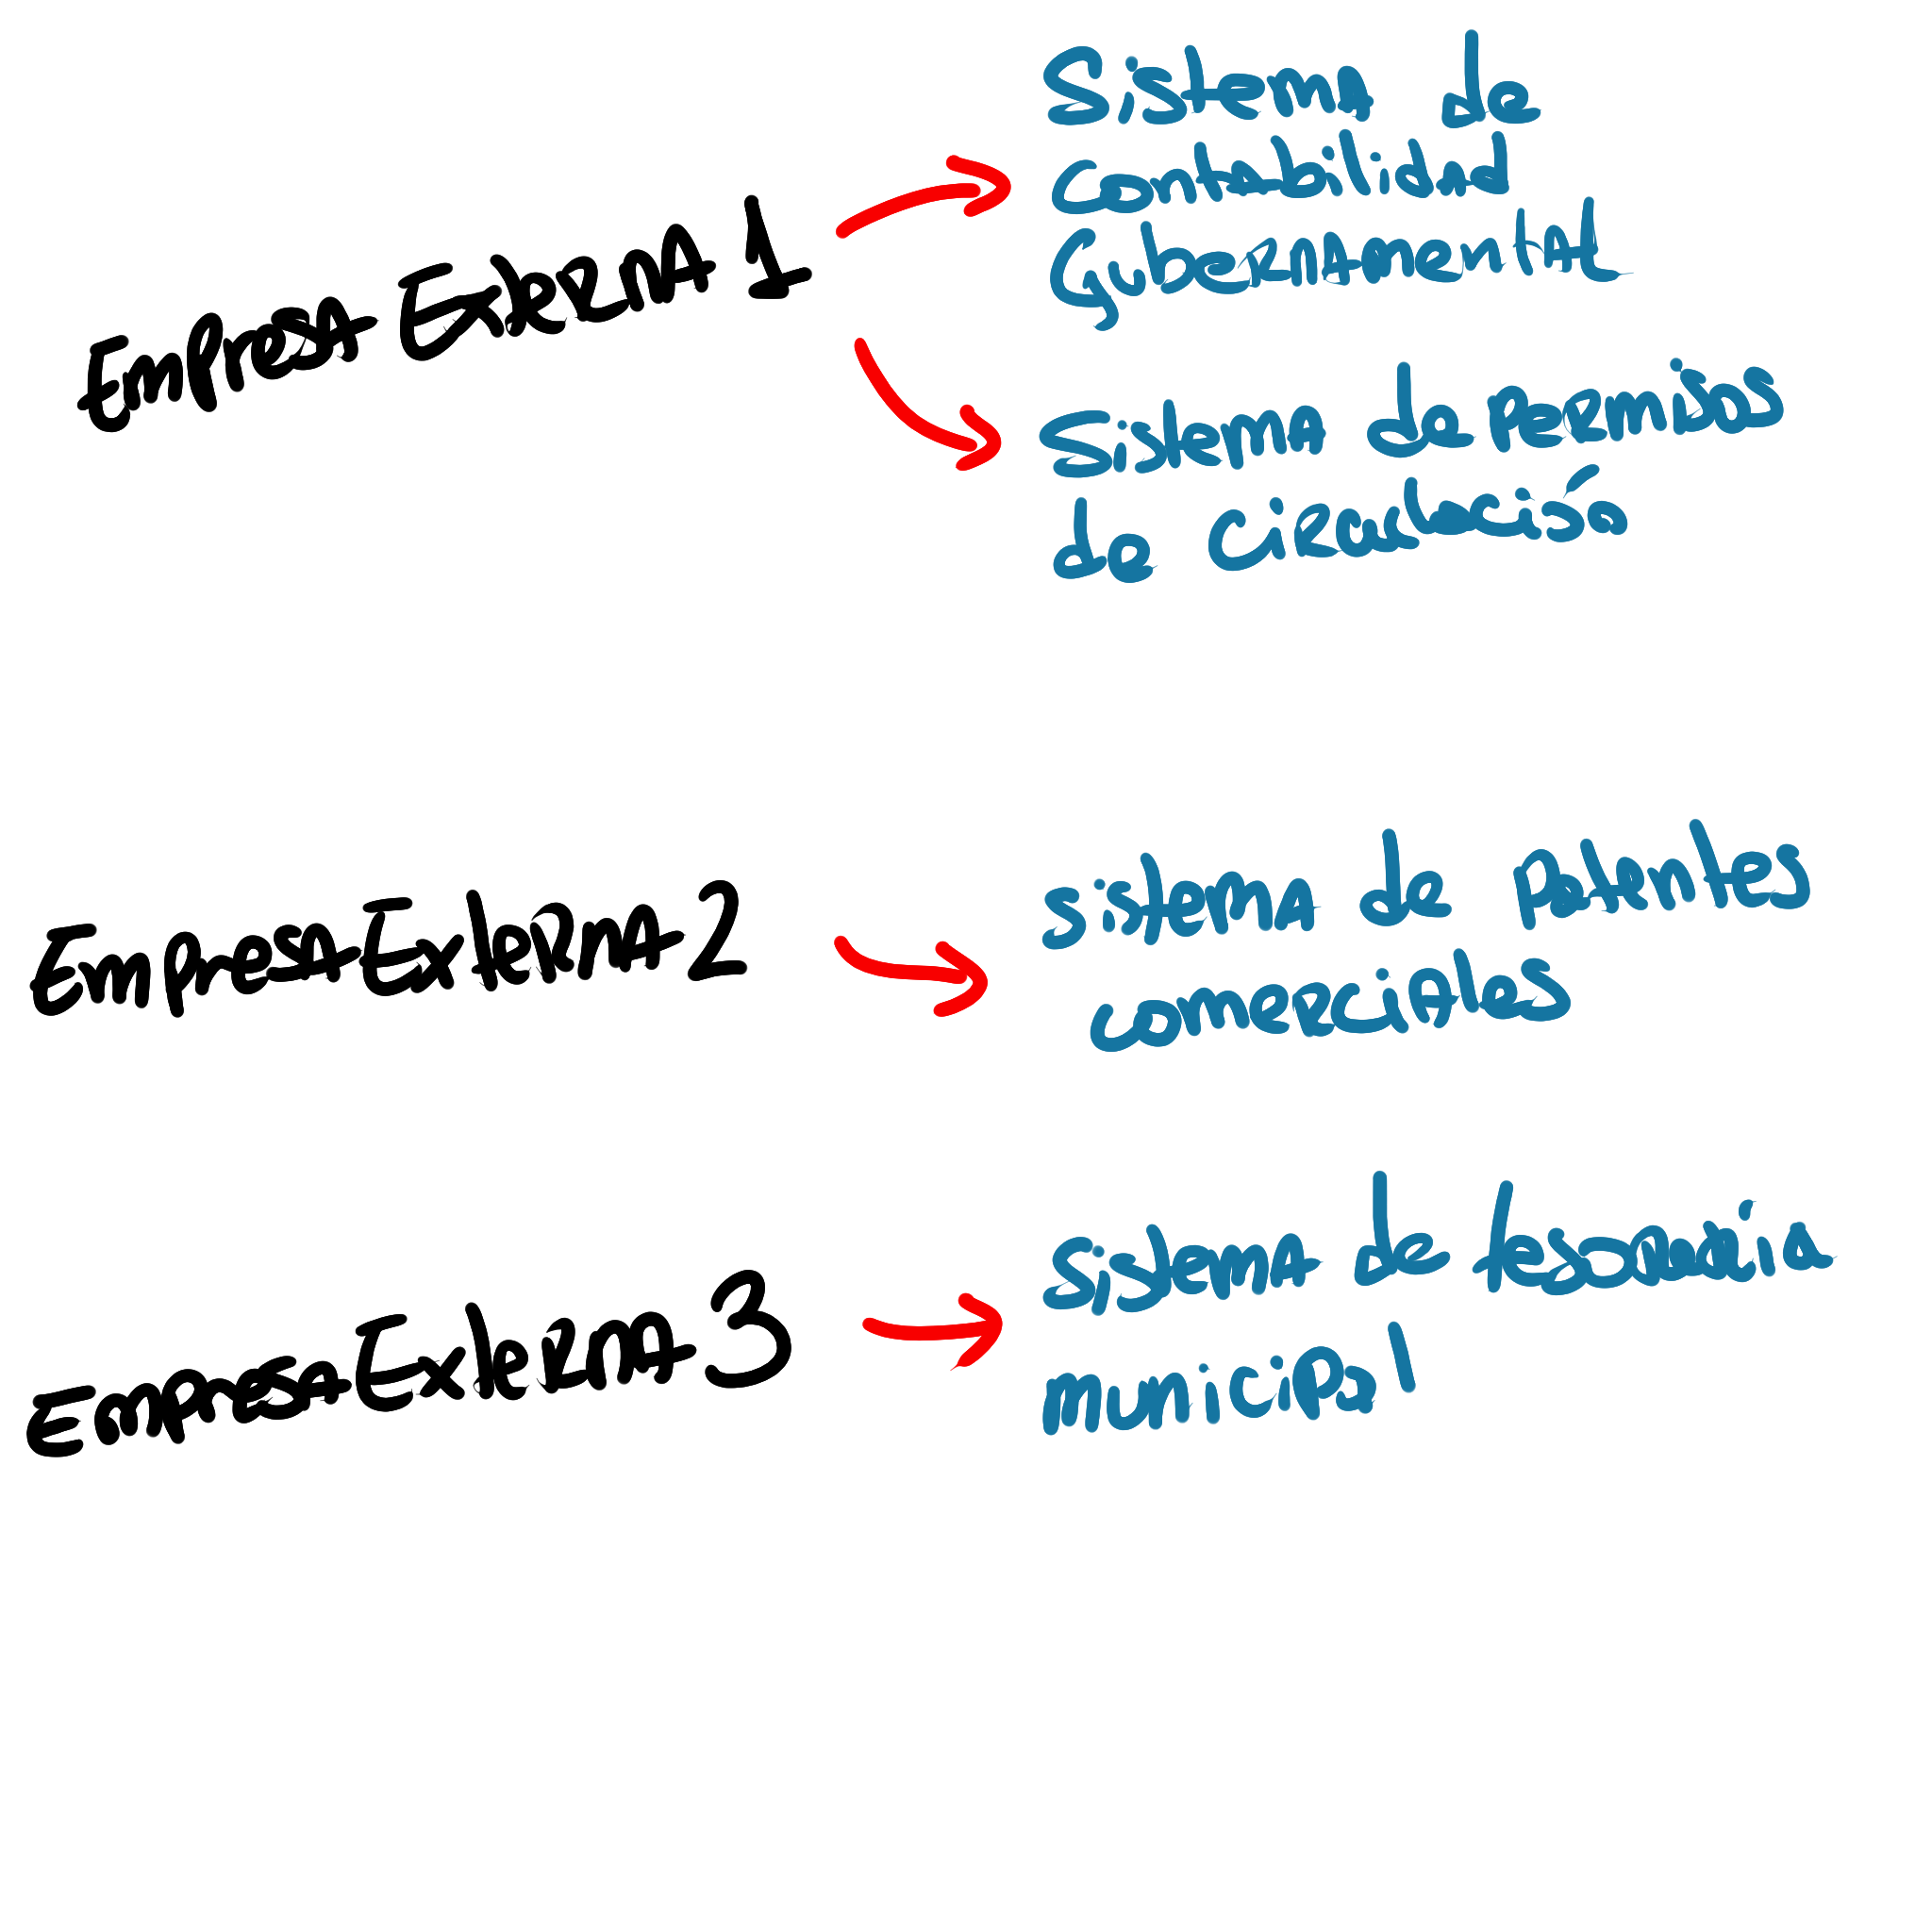
\includegraphics[width=.7\textwidth]{./images/6.png}\\
	\end{figure}
\end{frame}
\begin{frame}[c,fragile]
	\frametitle{Sistemas externalizados - Versión simple}
	\begin{figure}[H]
		\centering
		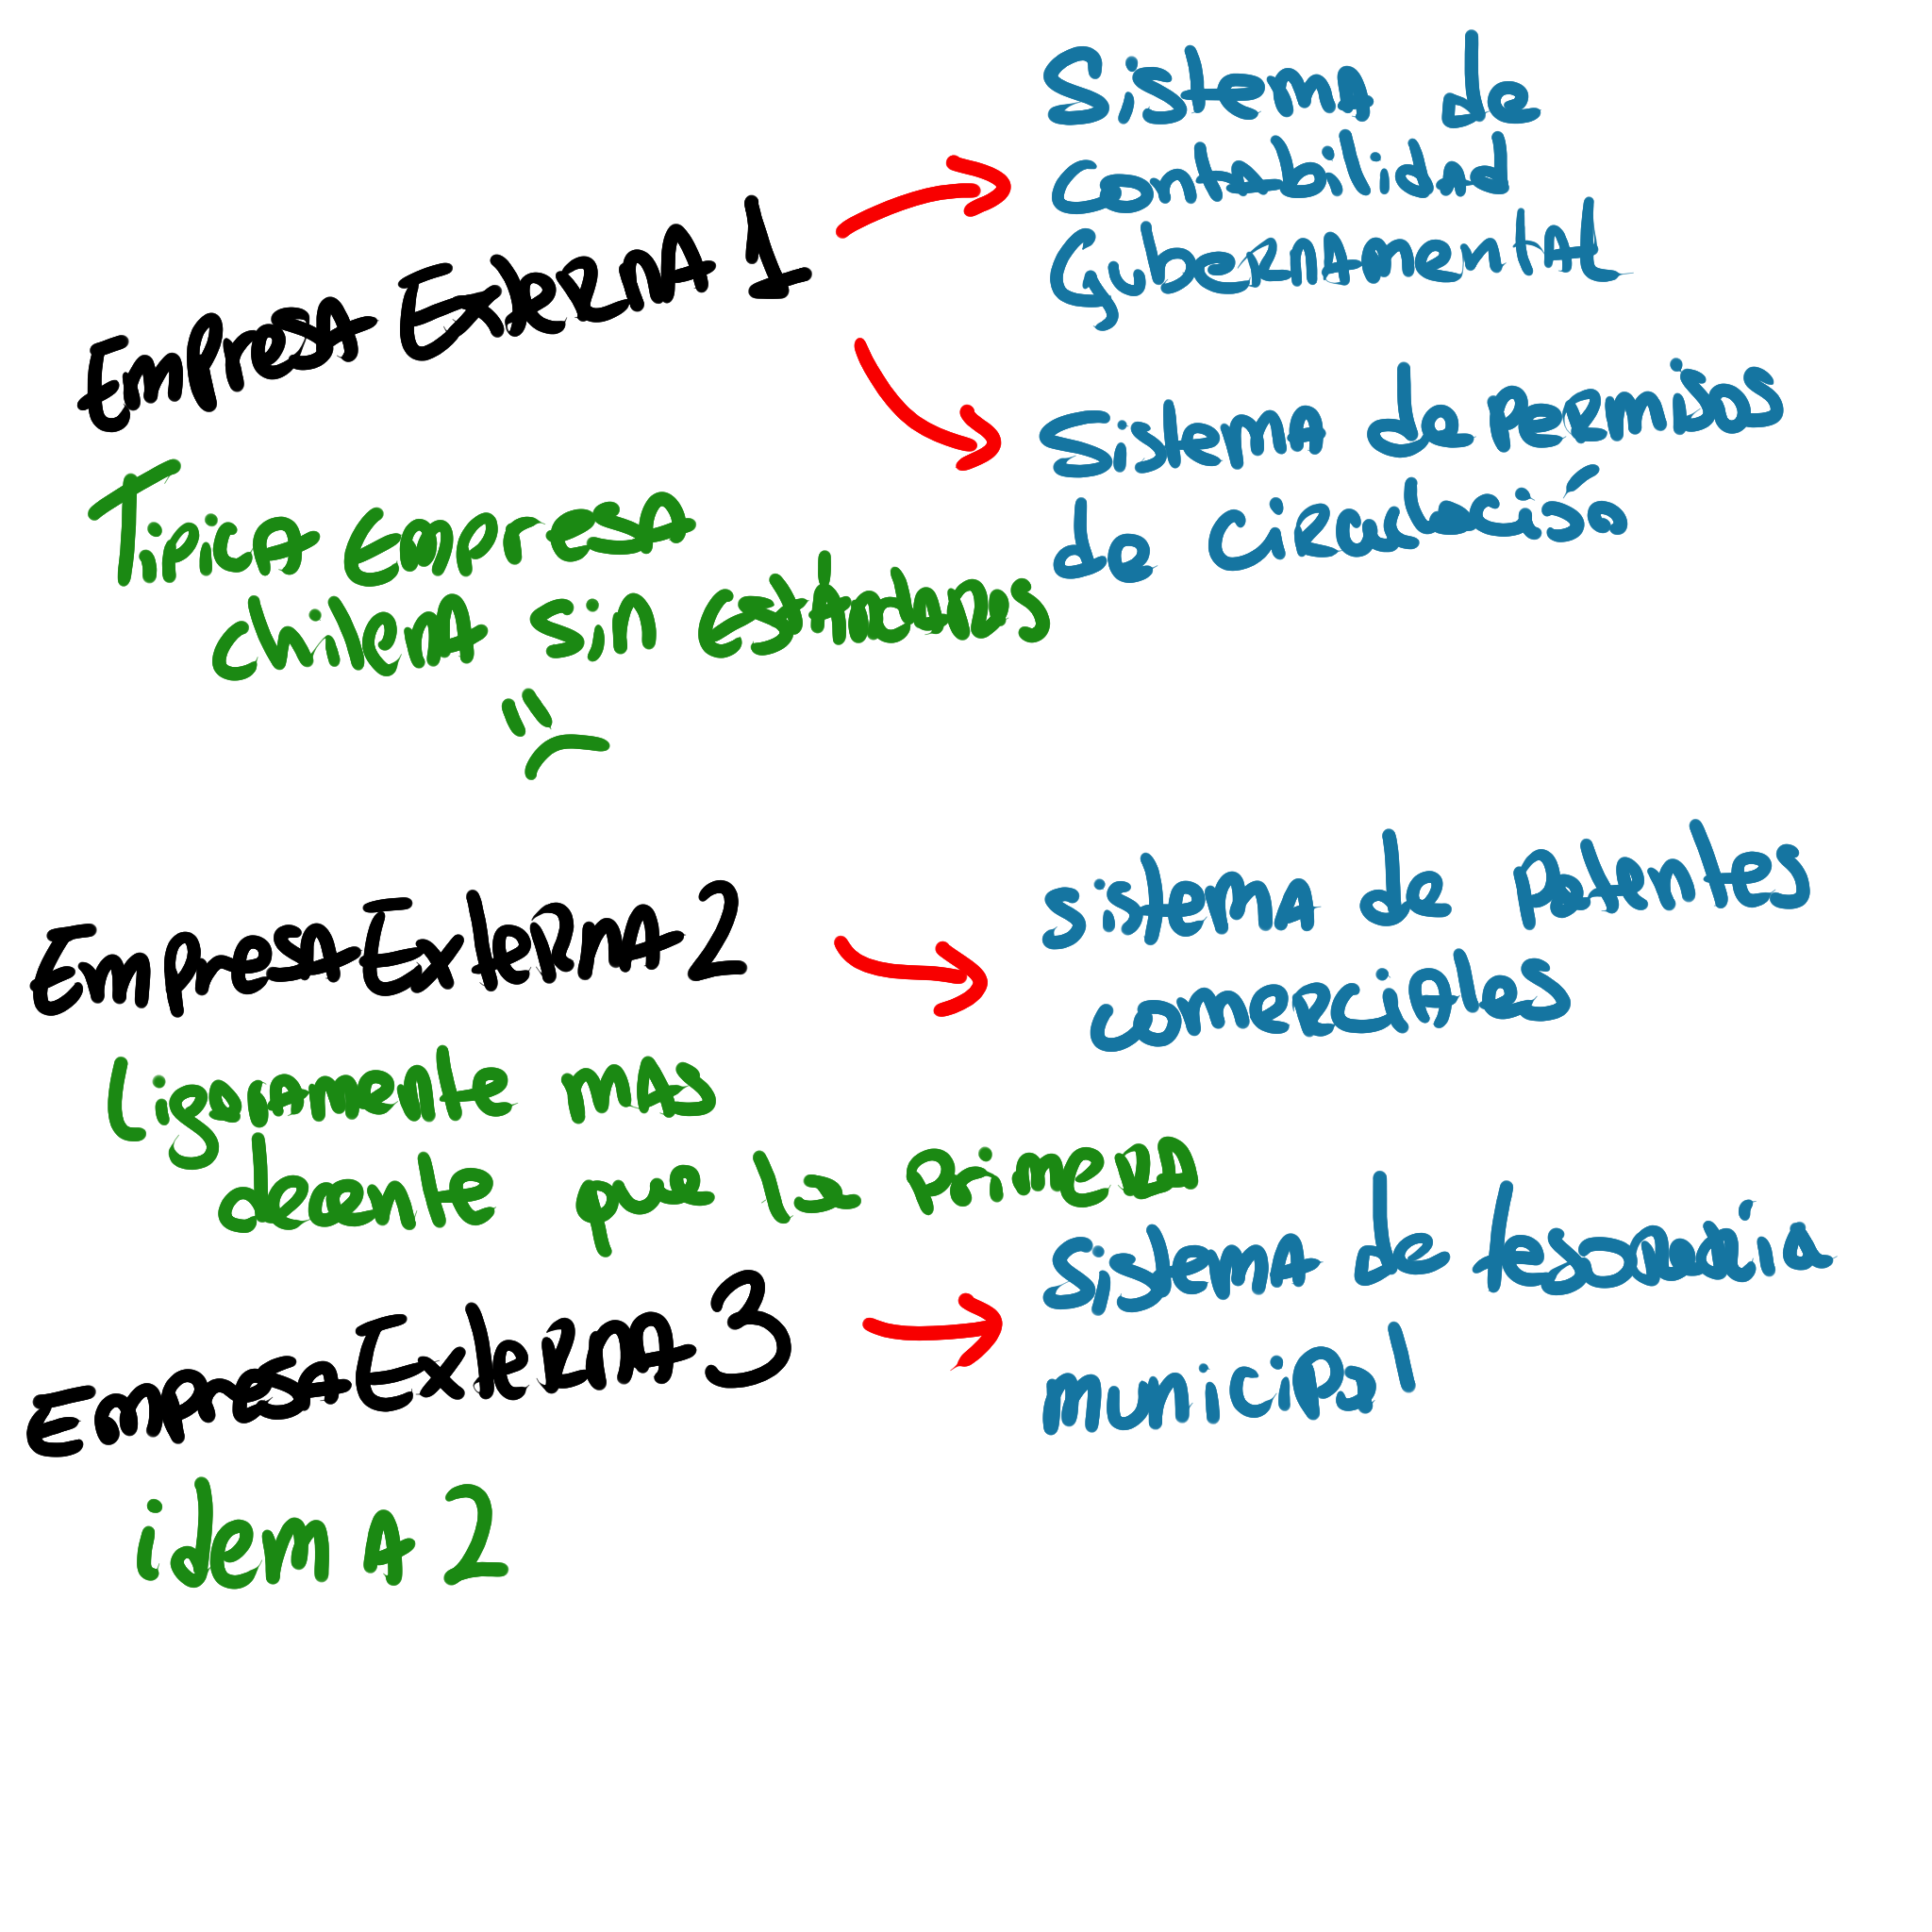
\includegraphics[width=.7\textwidth]{./images/7.png}\\
	\end{figure}
\end{frame}



\begin{frame}[c,fragile]
	\frametitle{Estructura de activos}
	\begin{itemize}
		\item{Sistemas}
		\item{Activos Transversales}
		\item{Activos Externalizados}
		\item{Activos Específicos}
	\end{itemize}
\end{frame}

\begin{frame}[c,fragile]
	\frametitle{Estructura de los activos - Simplificado}
	\begin{figure}[H]
		\centering
		
\includegraphics[width=.7\textwidth]{./auditoria/1.png}\\
	\end{figure}
\end{frame}

\begin{frame}[c,fragile]
	\frametitle{Estructura de los activos - Simplificado}
	\begin{figure}[H]
		\centering
		
\includegraphics[width=.7\textwidth]{./auditoria/2.png}\\
	\end{figure}
\end{frame}

\begin{frame}[c,fragile]
	\frametitle{Estructura de los activos - Simplificado}
	\begin{figure}[H]
		\centering
		
\includegraphics[width=.7\textwidth]{./auditoria/3.png}\\
	\end{figure}
\end{frame}

\begin{frame}[c,fragile]
	\frametitle{Estructura de los activos - Simplificado}
	\begin{figure}[H]
		\centering
		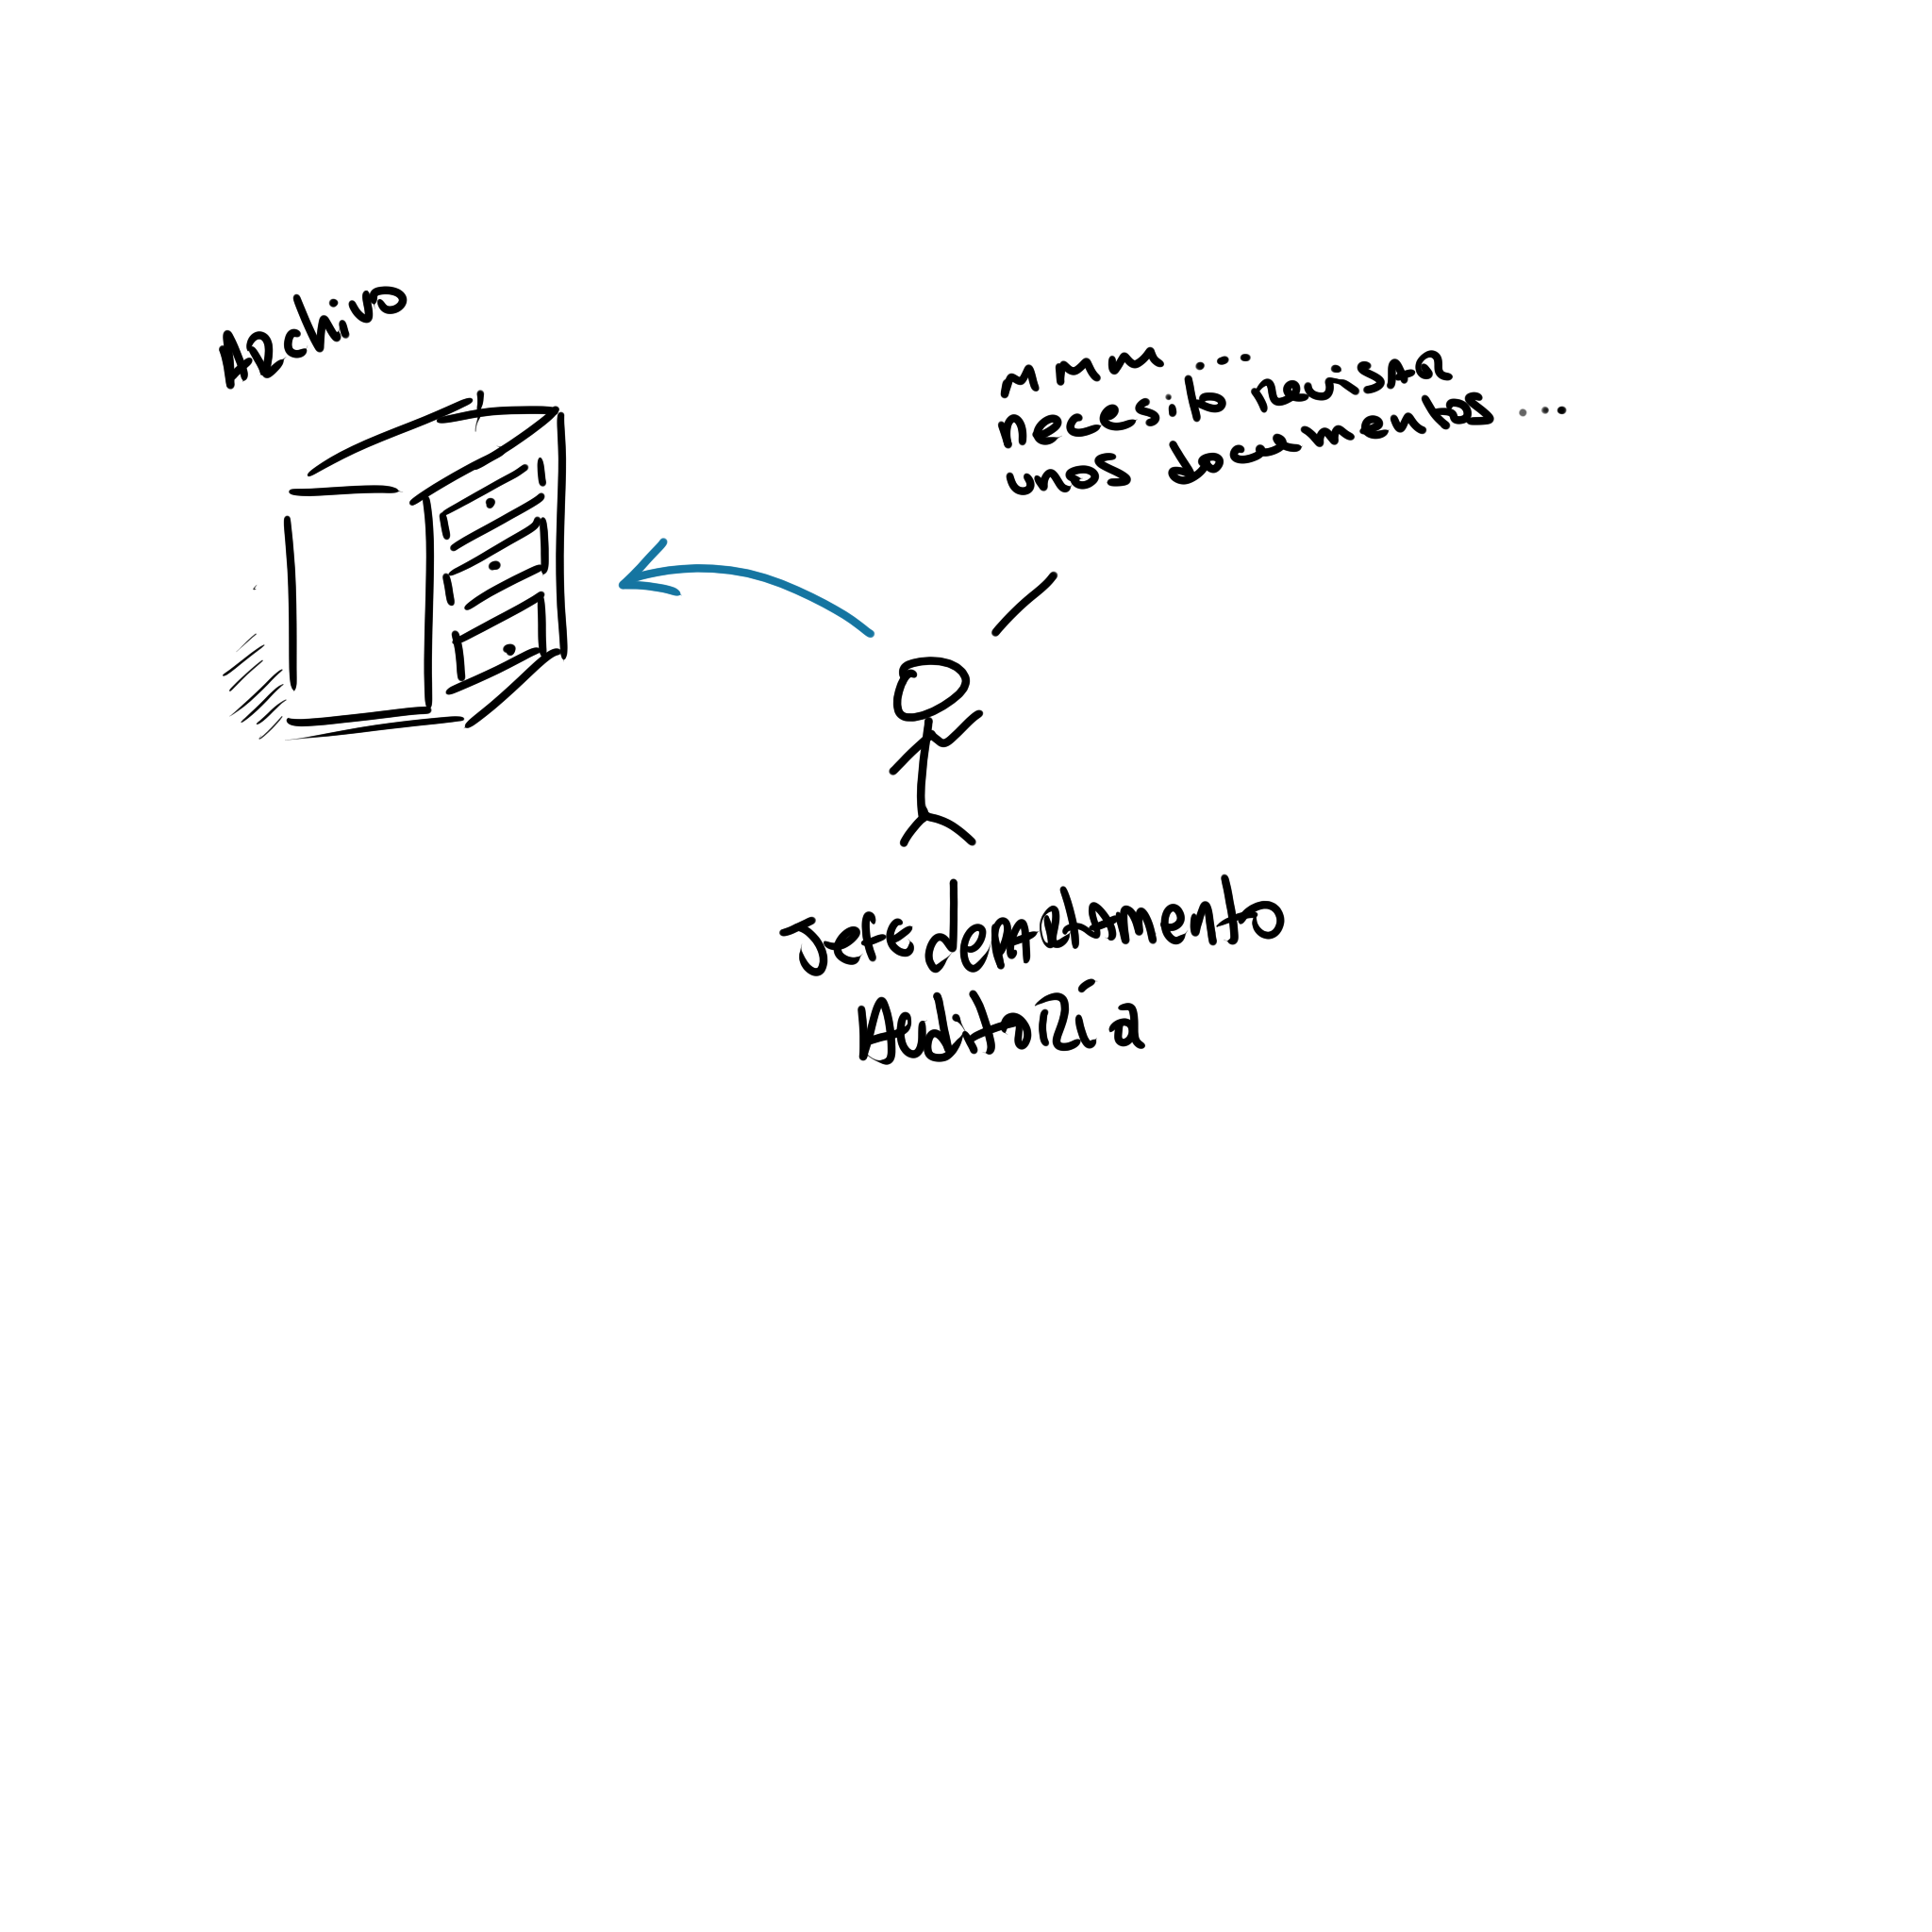
\includegraphics[width=.7\textwidth]{./auditoria/4.png}\\
	\end{figure}
\end{frame}

\begin{frame}[c,fragile]
	\frametitle{Estructura de los activos - Simplificado}
	\begin{figure}[H]
		\centering
		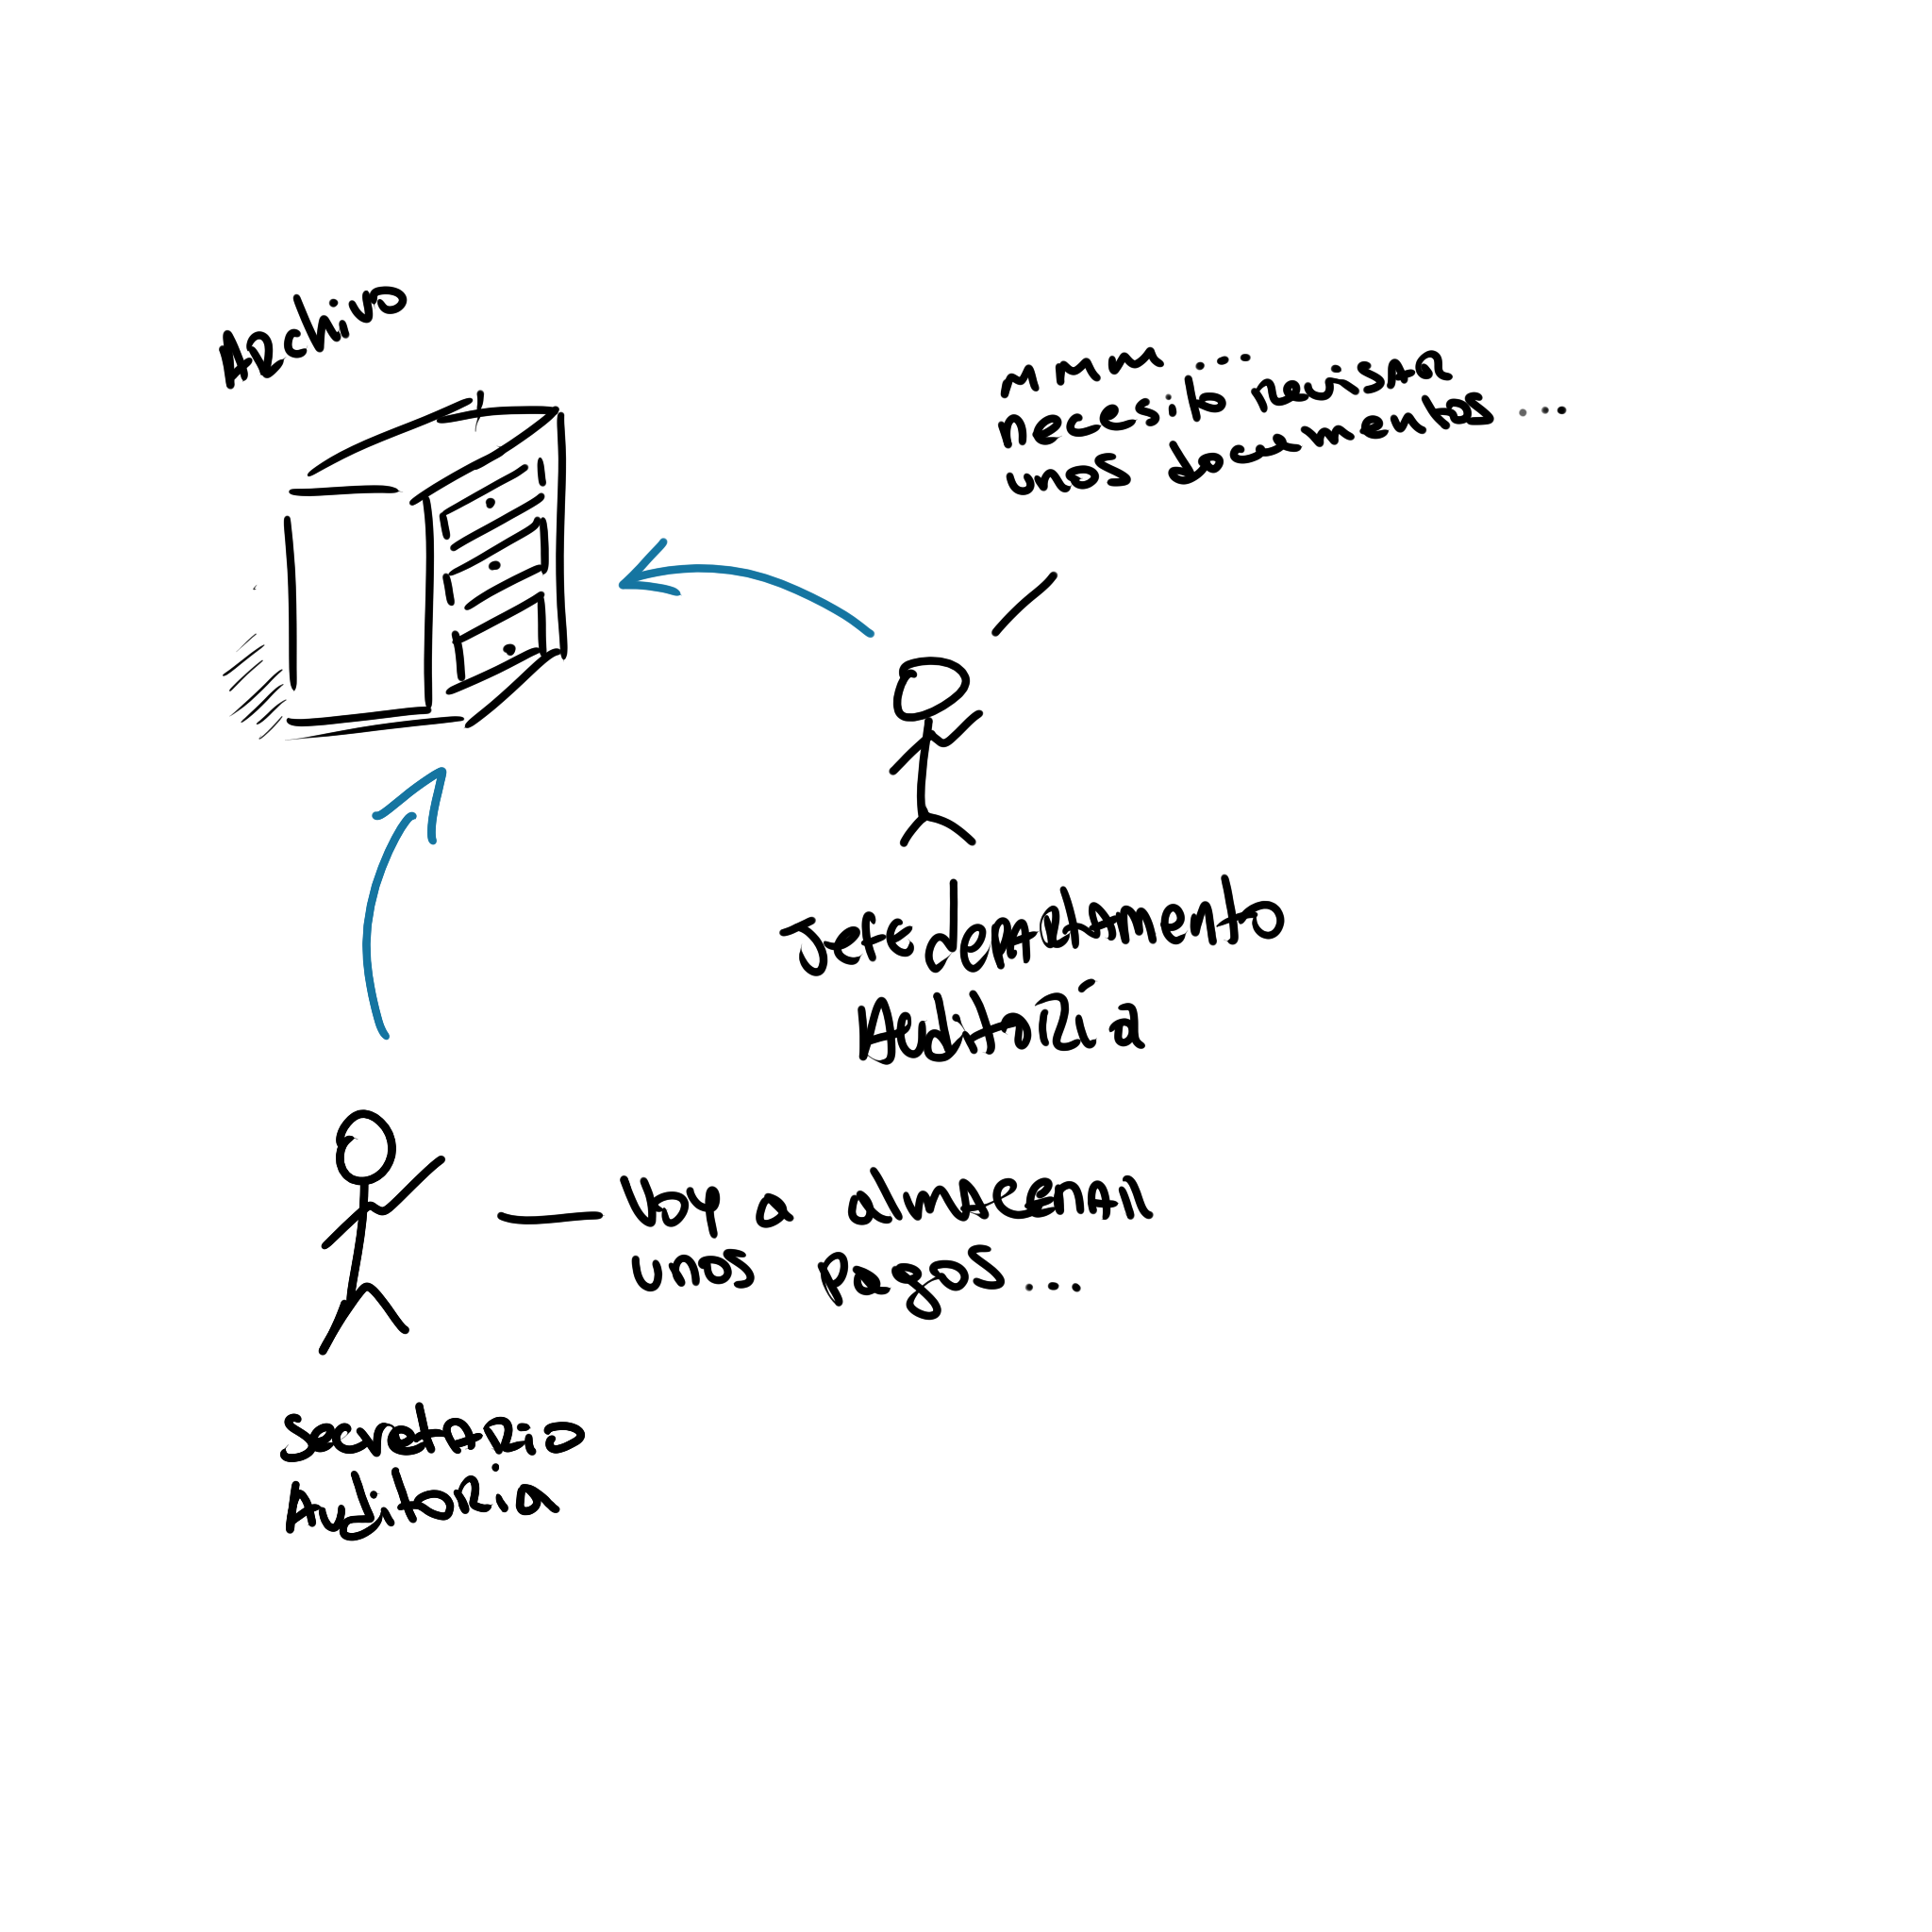
\includegraphics[width=.7\textwidth]{./auditoria/5.png}\\
	\end{figure}
\end{frame}

\begin{frame}[c,fragile]
	\frametitle{Estructura de los activos - Simplificado}
	\begin{figure}[H]
		\centering
		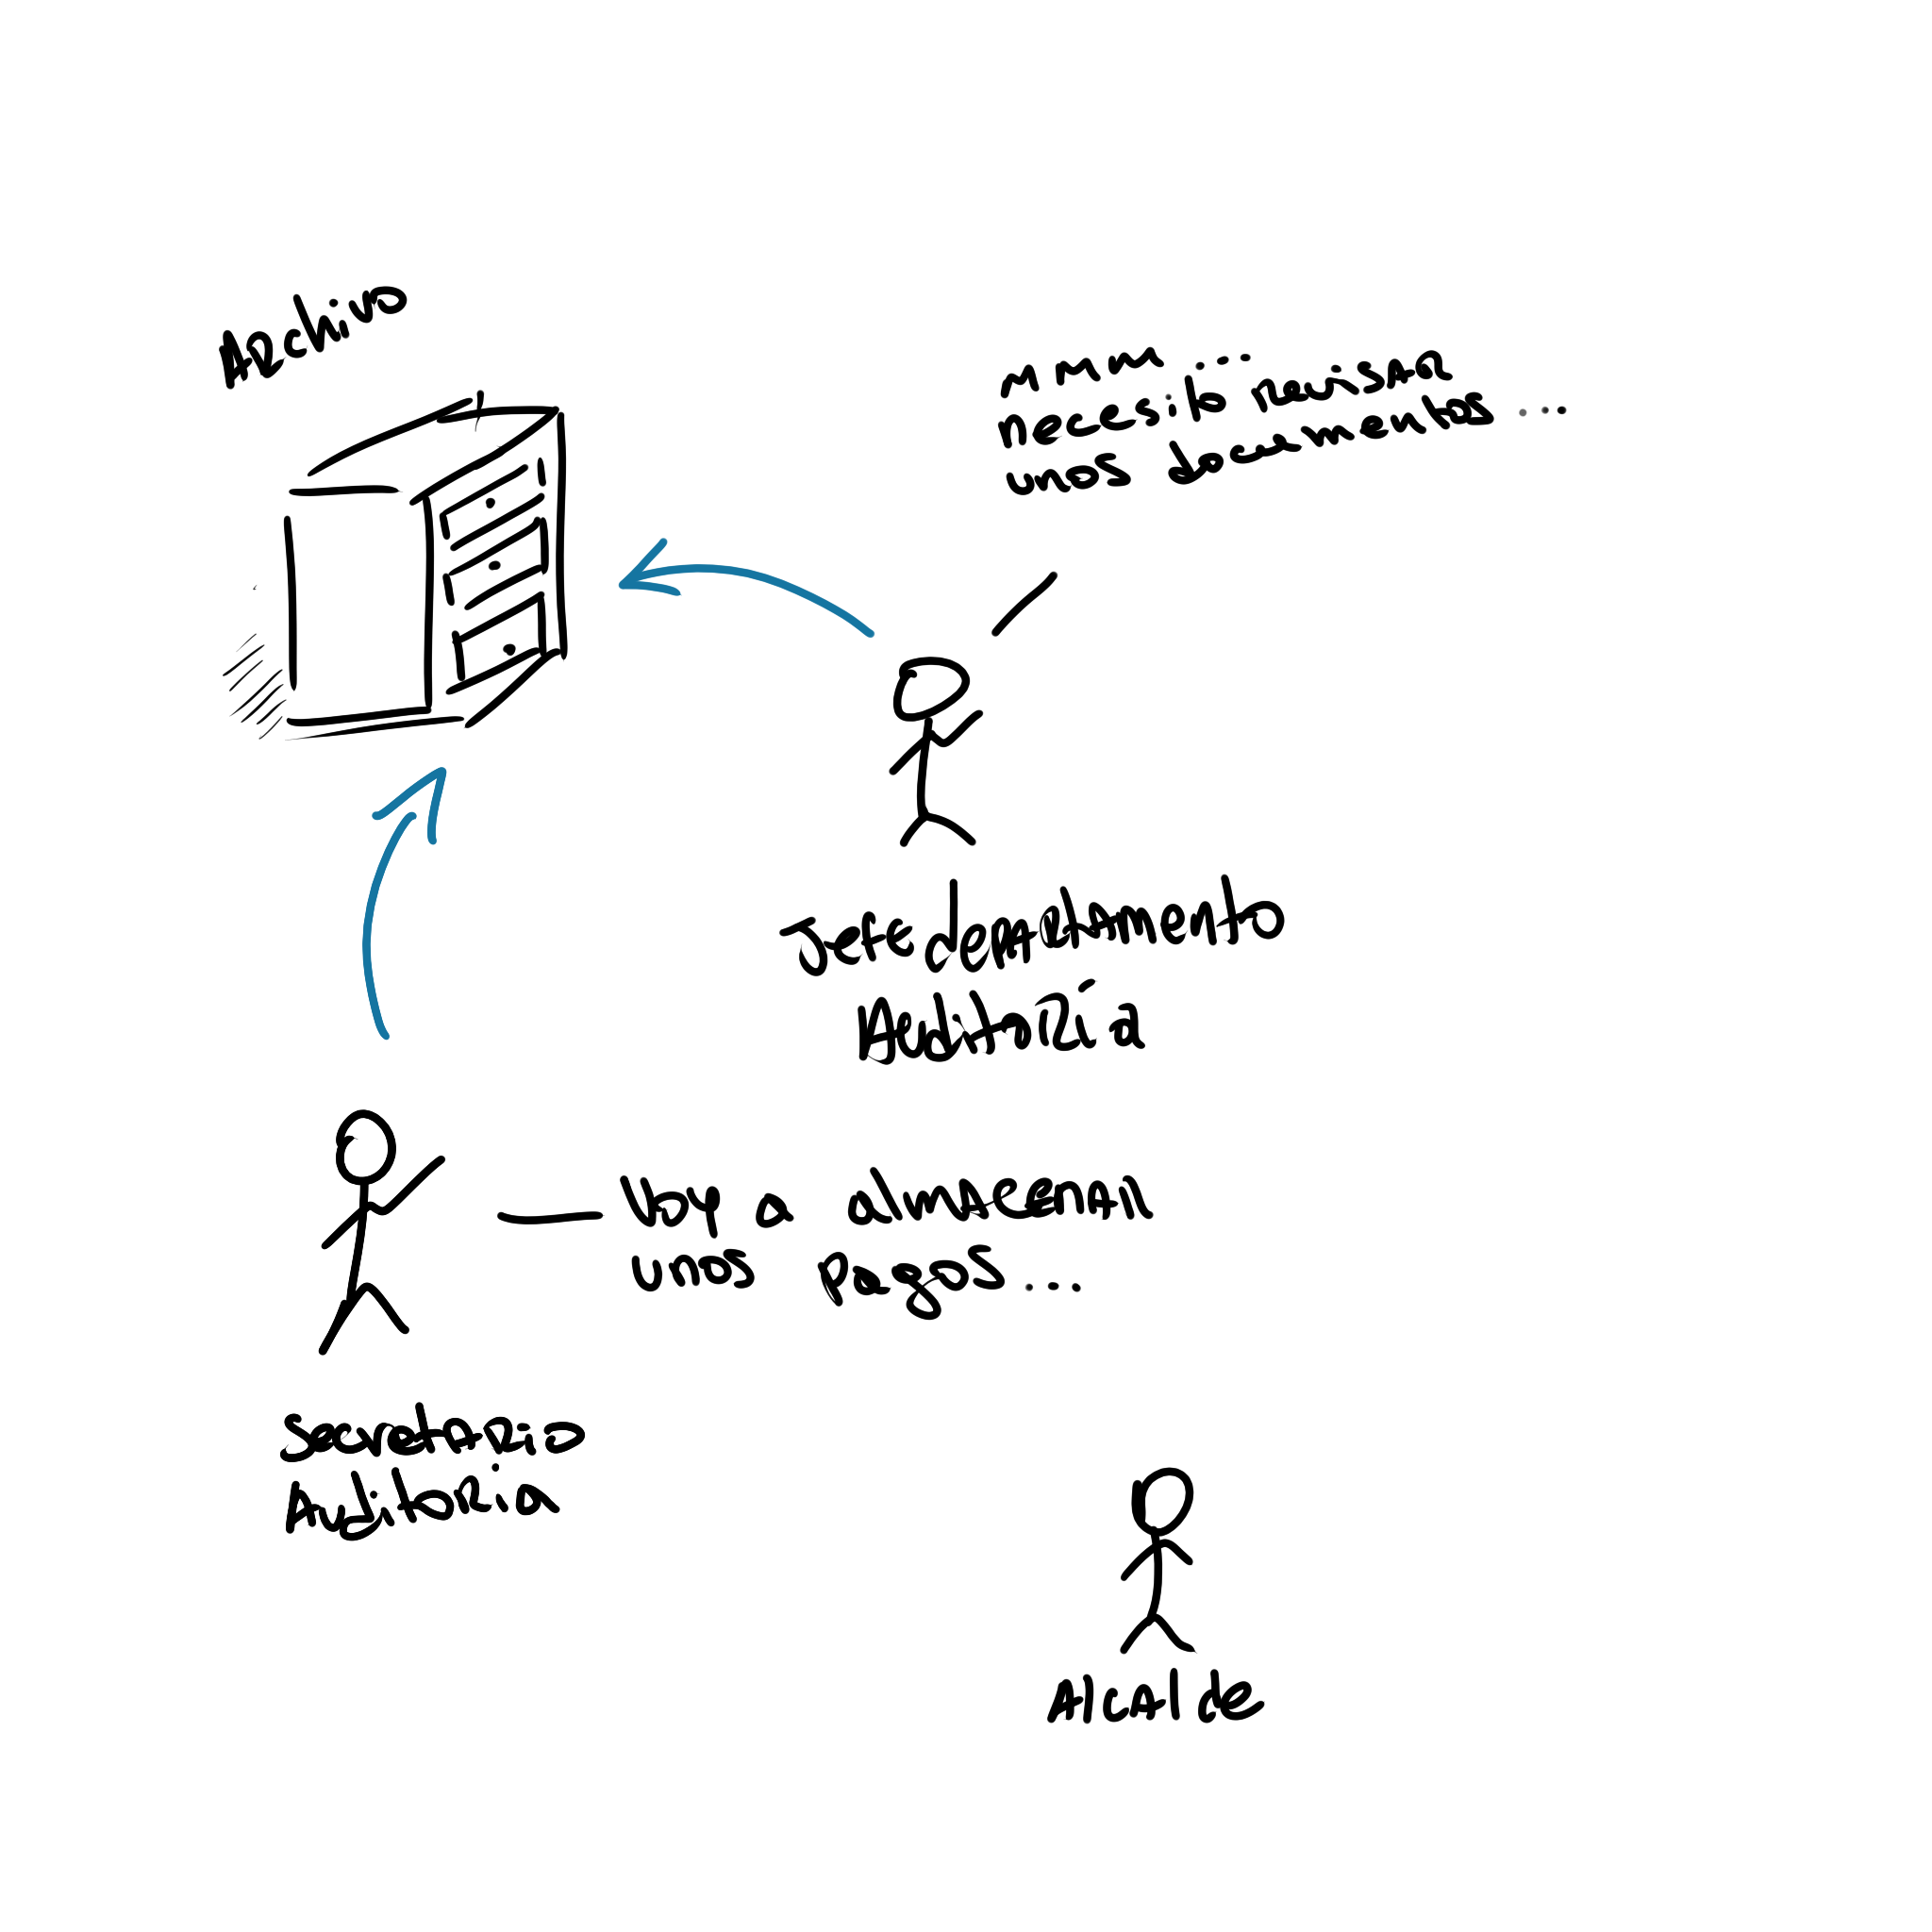
\includegraphics[width=.7\textwidth]{./auditoria/6.png}\\
	\end{figure}
\end{frame}

\begin{frame}[c,fragile]
	\frametitle{Estructura de los activos - Simplificado}
	\begin{figure}[H]
		\centering
		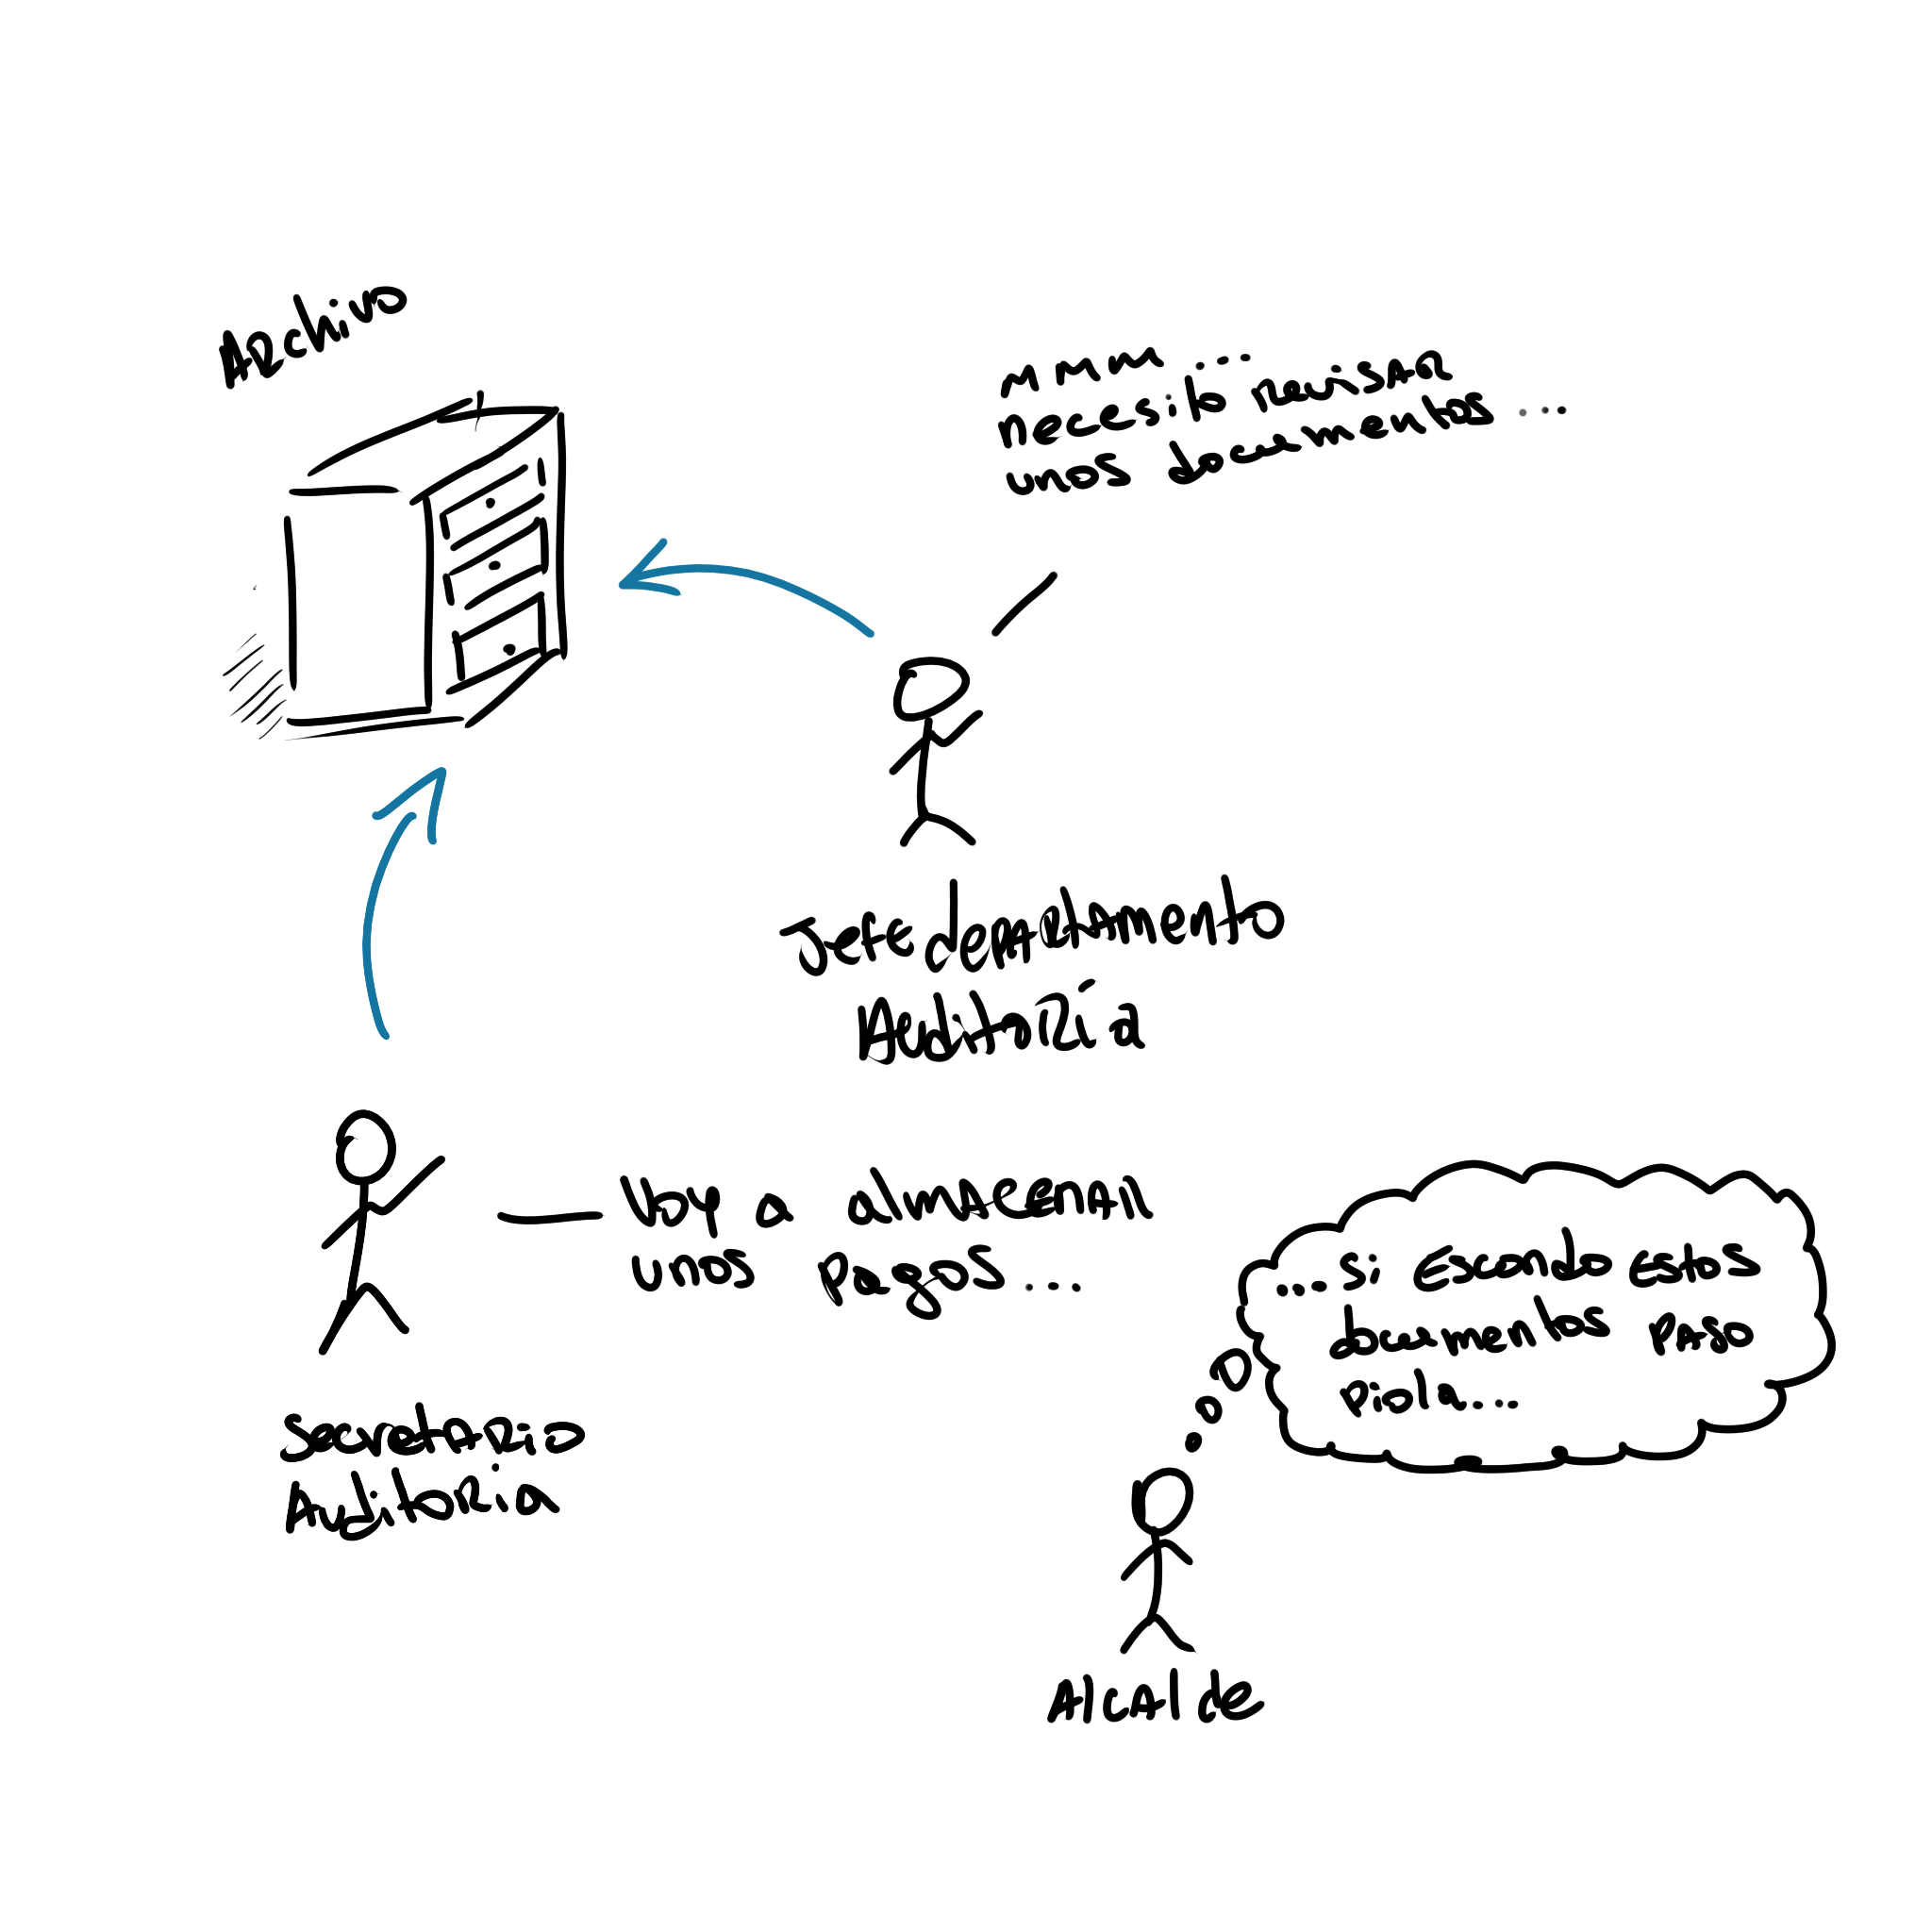
\includegraphics[width=.7\textwidth]{./auditoria/7.png}\\
	\end{figure}
\end{frame}

\begin{frame}[c,fragile]
	\frametitle{Estructura de los activos - Simplificado}
	\begin{figure}[H]
		\centering
		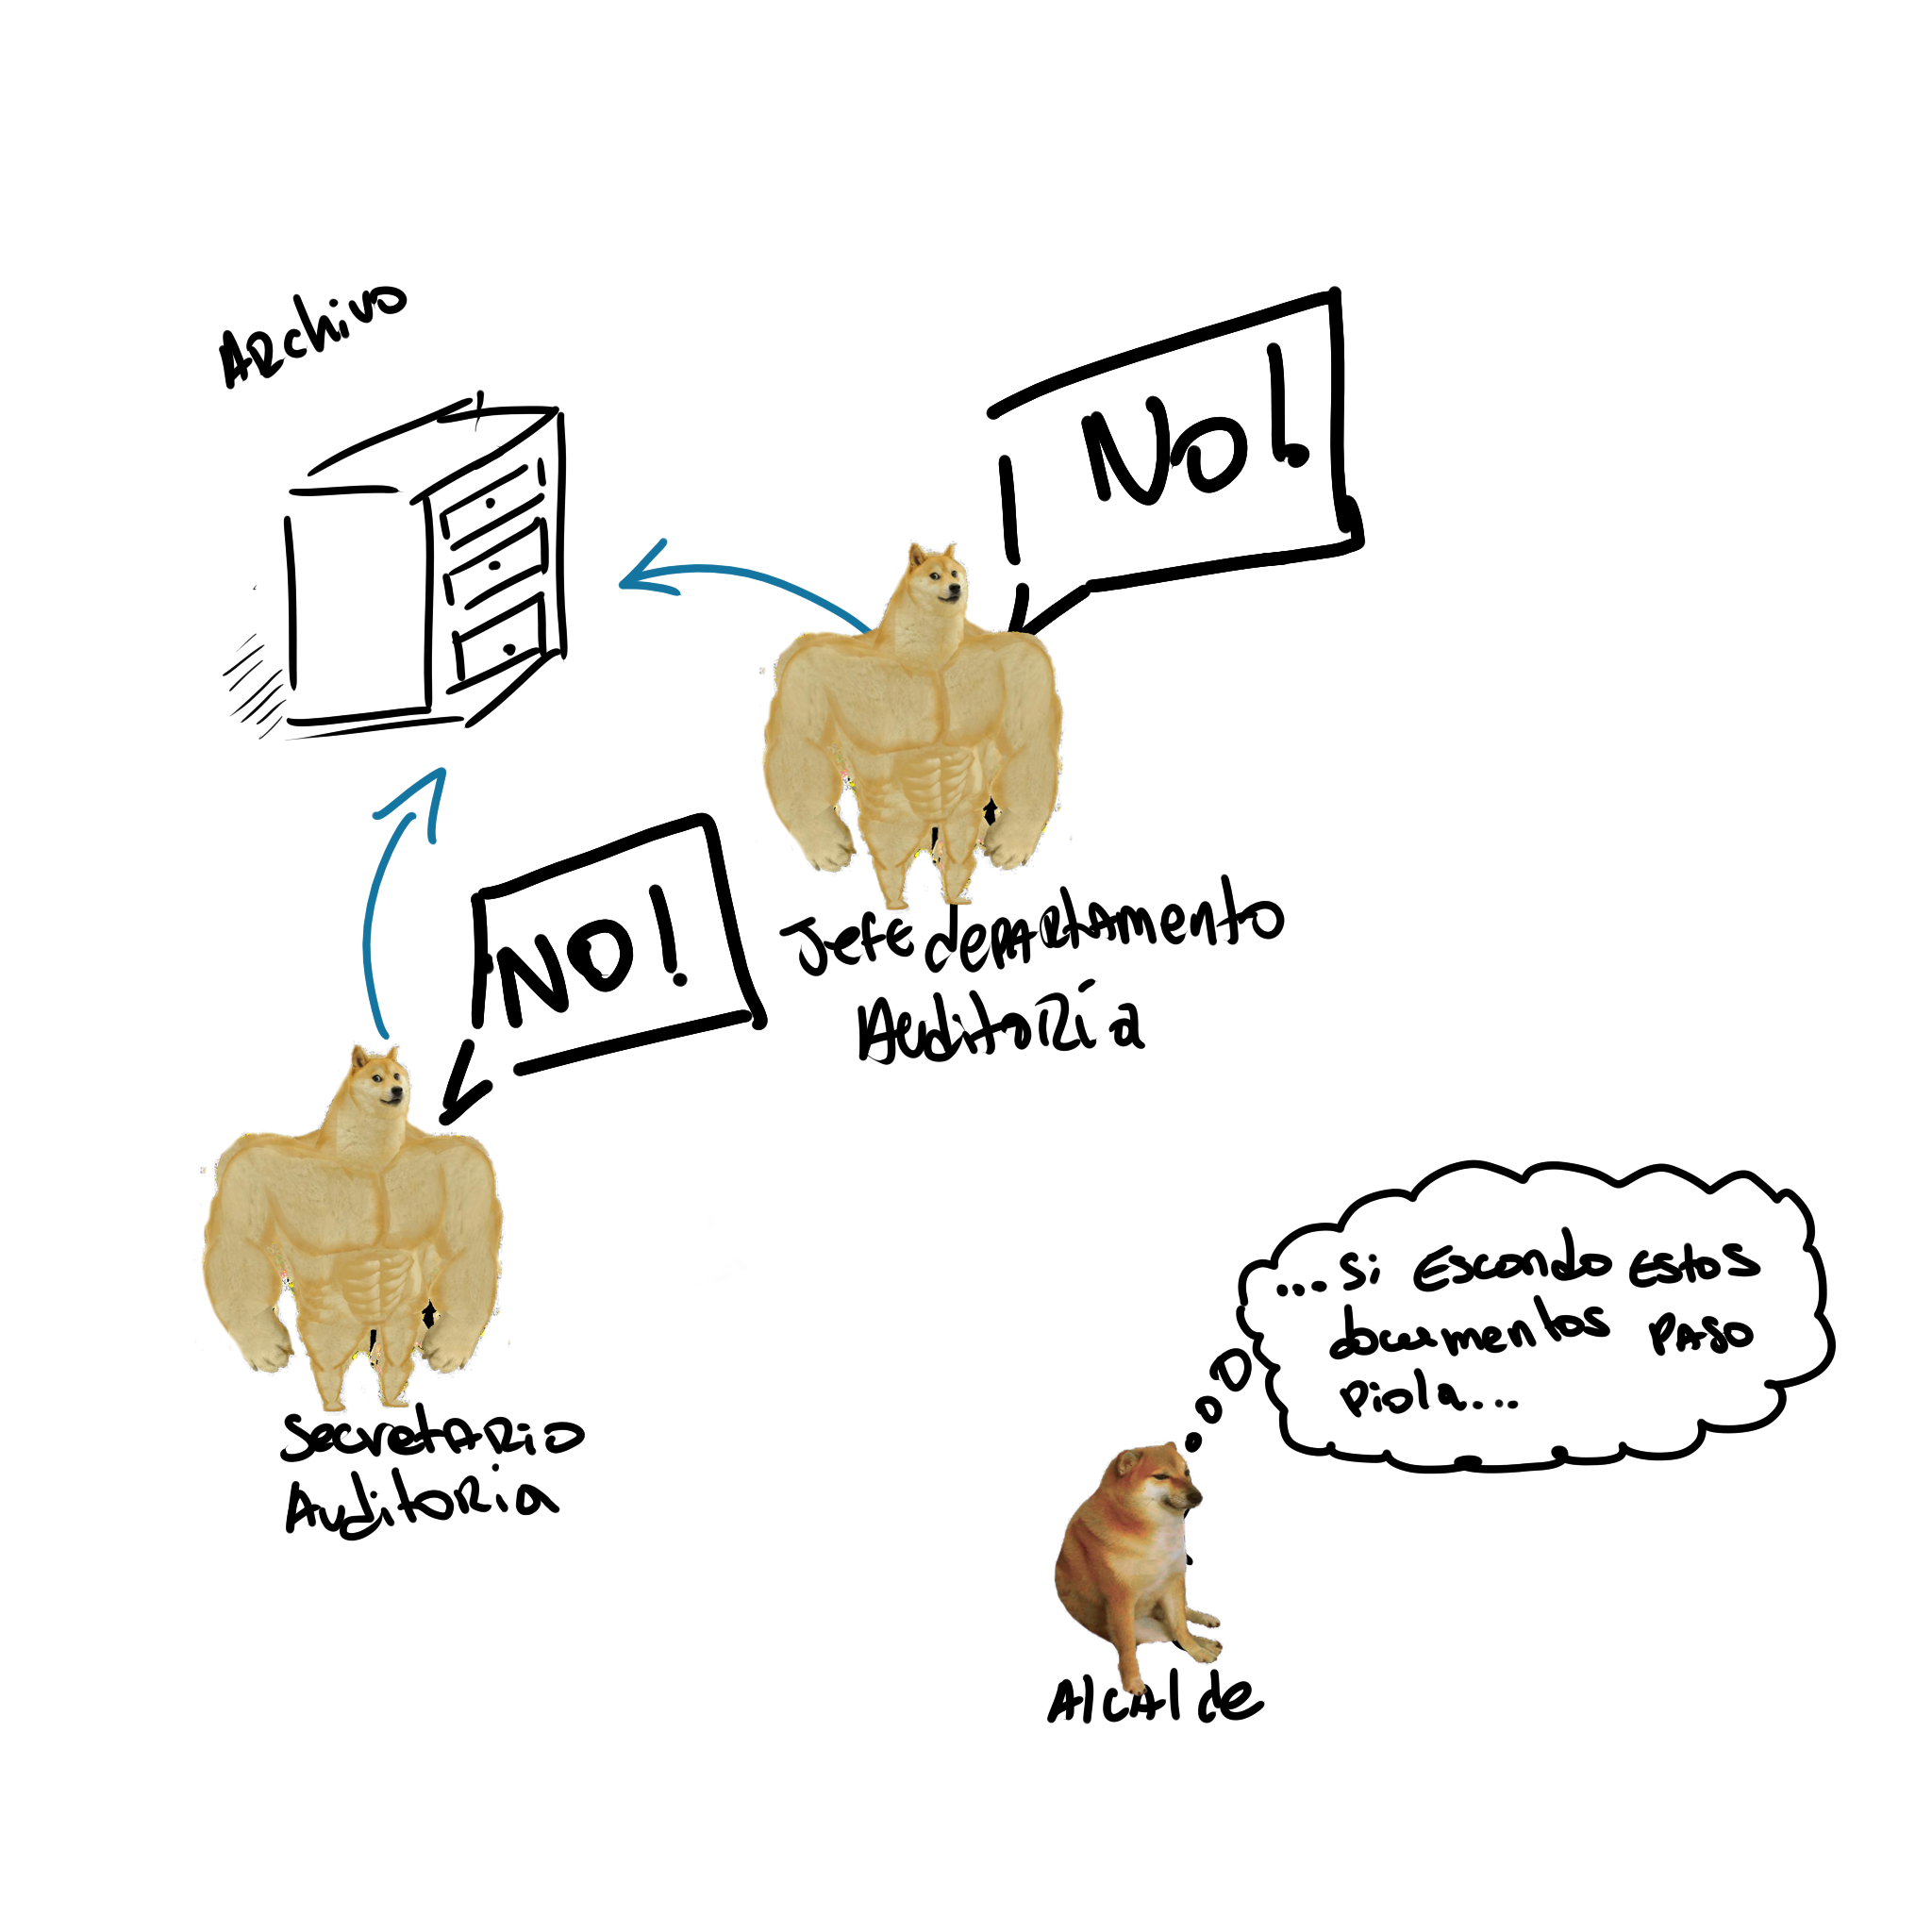
\includegraphics[width=.7\textwidth]{./auditoria/8.png}\\
	\end{figure}
\end{frame}

\begin{frame}[c,fragile]
	\frametitle{Estructura de los activos - Simplificado}
	\begin{figure}[H]
		\centering
		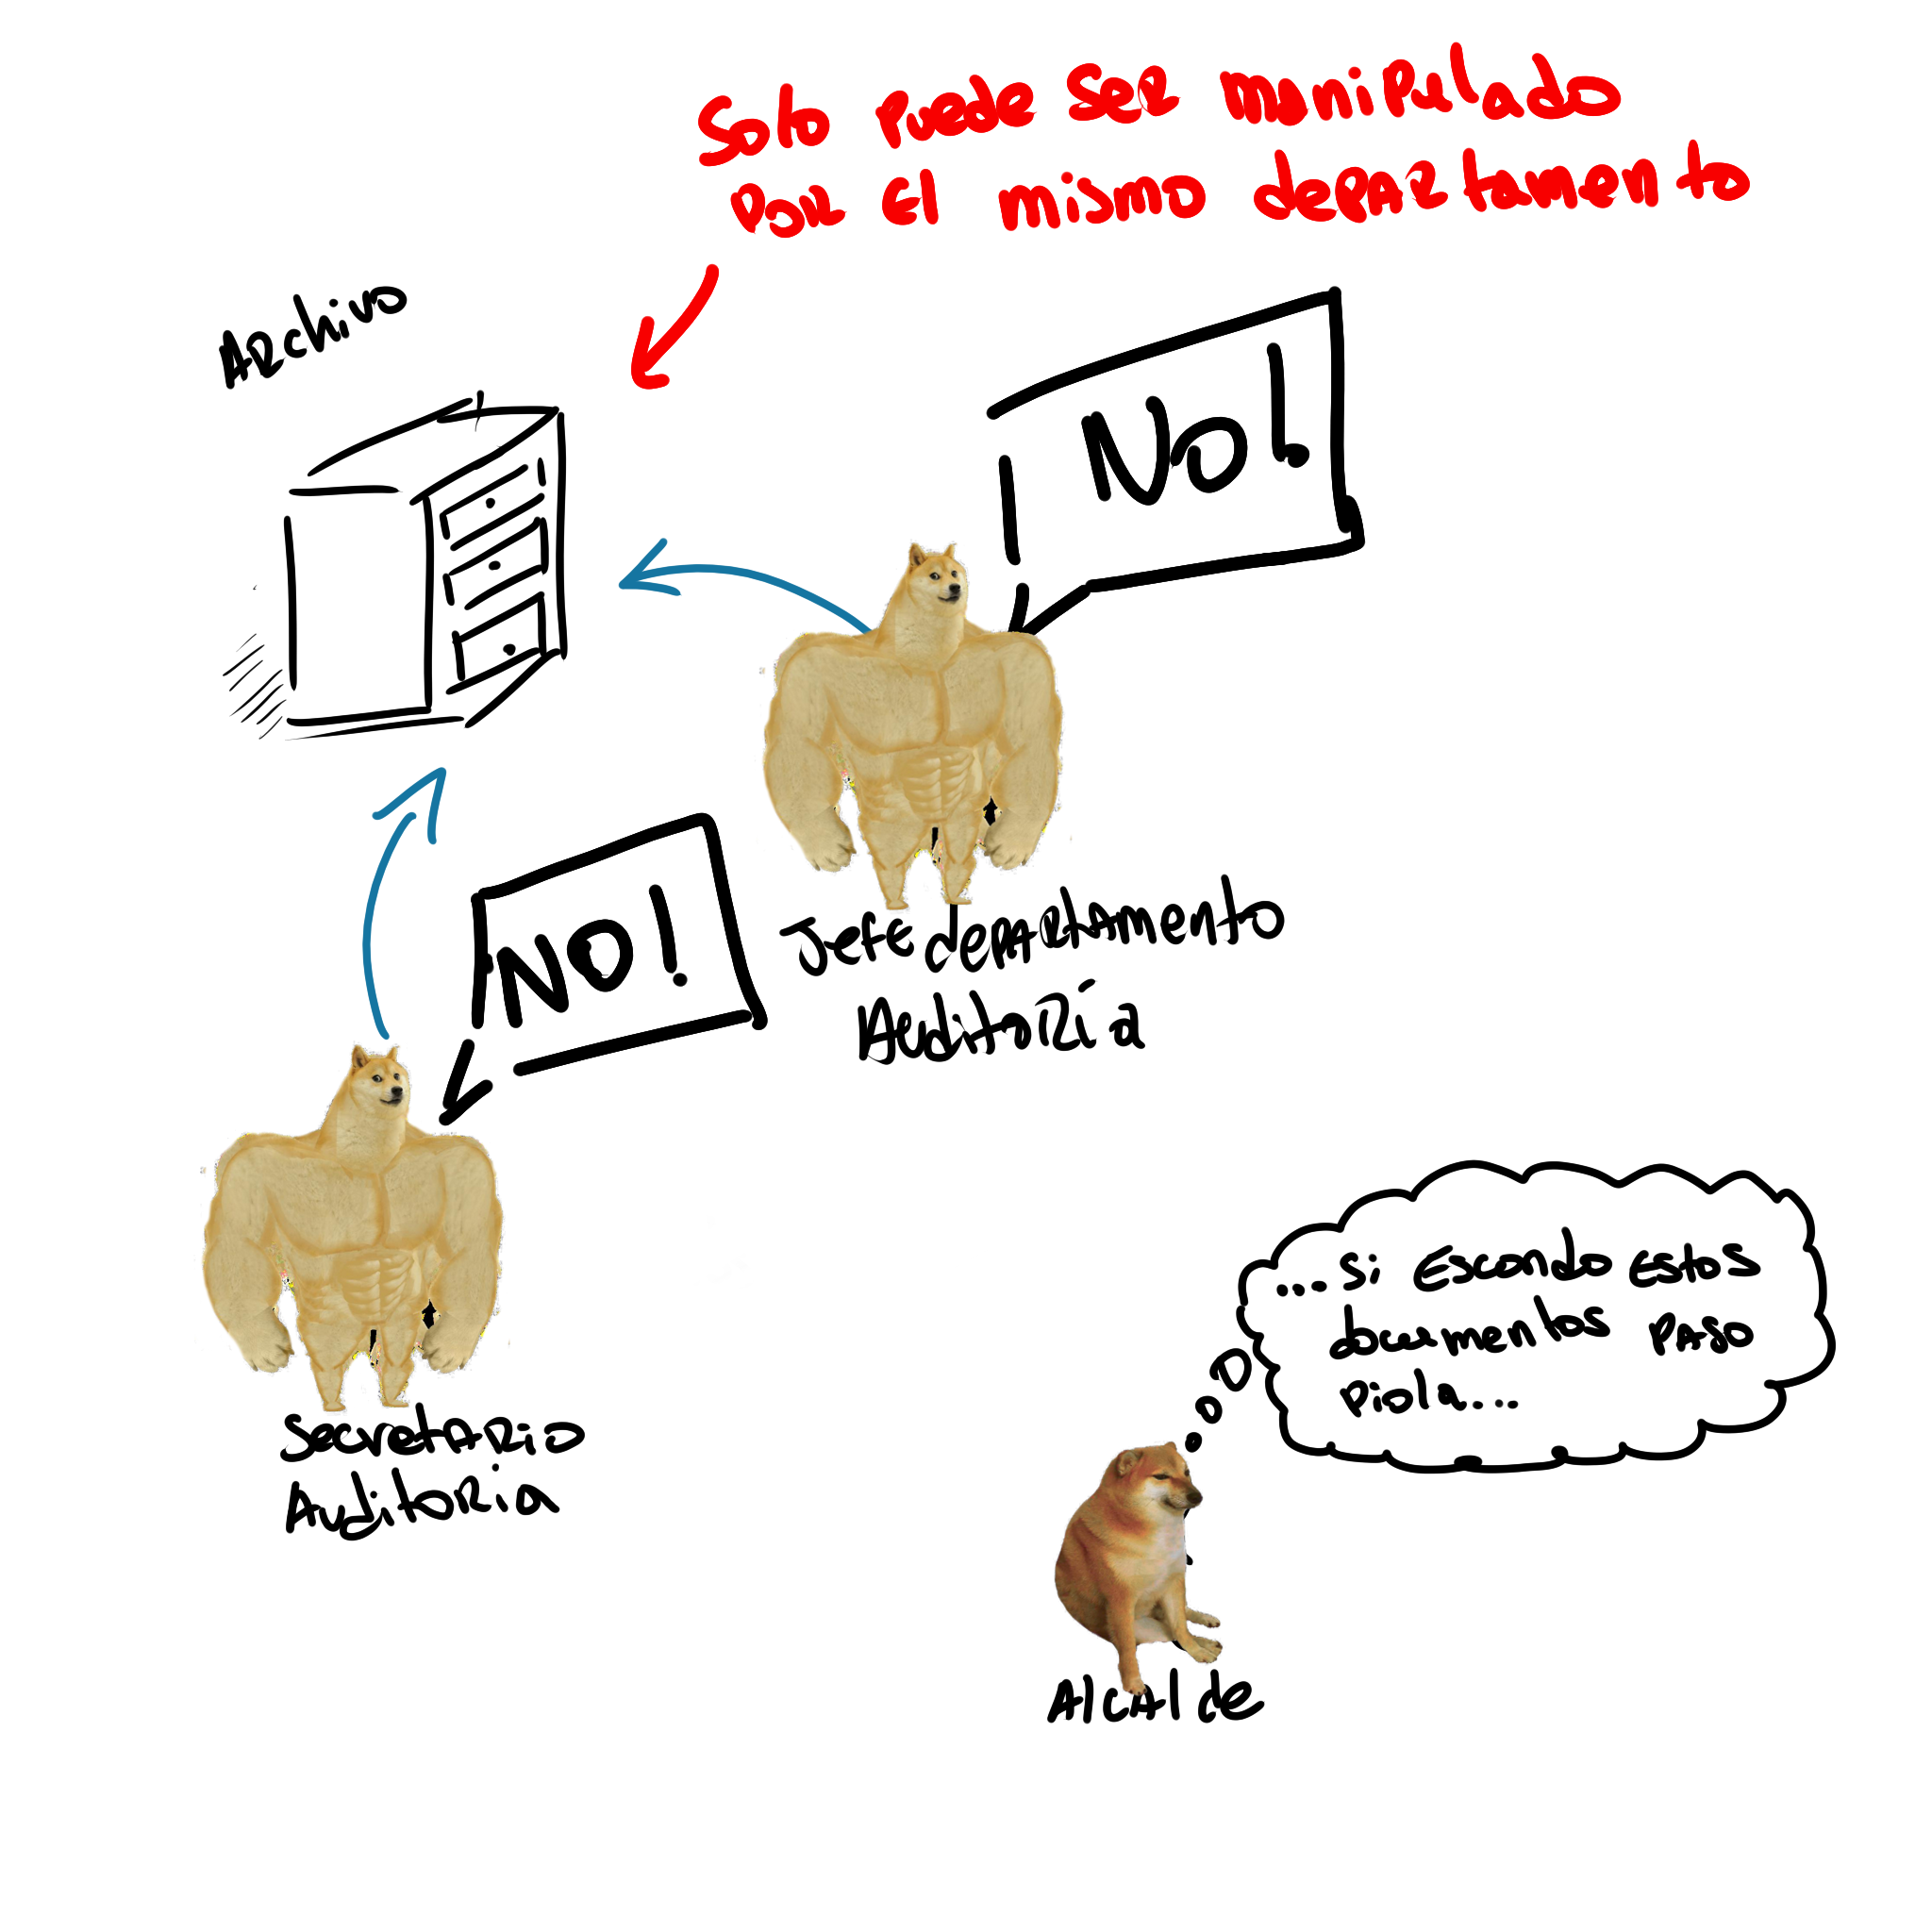
\includegraphics[width=.7\textwidth]{./auditoria/9.png}\\
	\end{figure}
\end{frame}

\begin{frame}[c,fragile]
	\frametitle{Estructura de los activos - Simplificado}
	\begin{figure}[H]
		\centering
		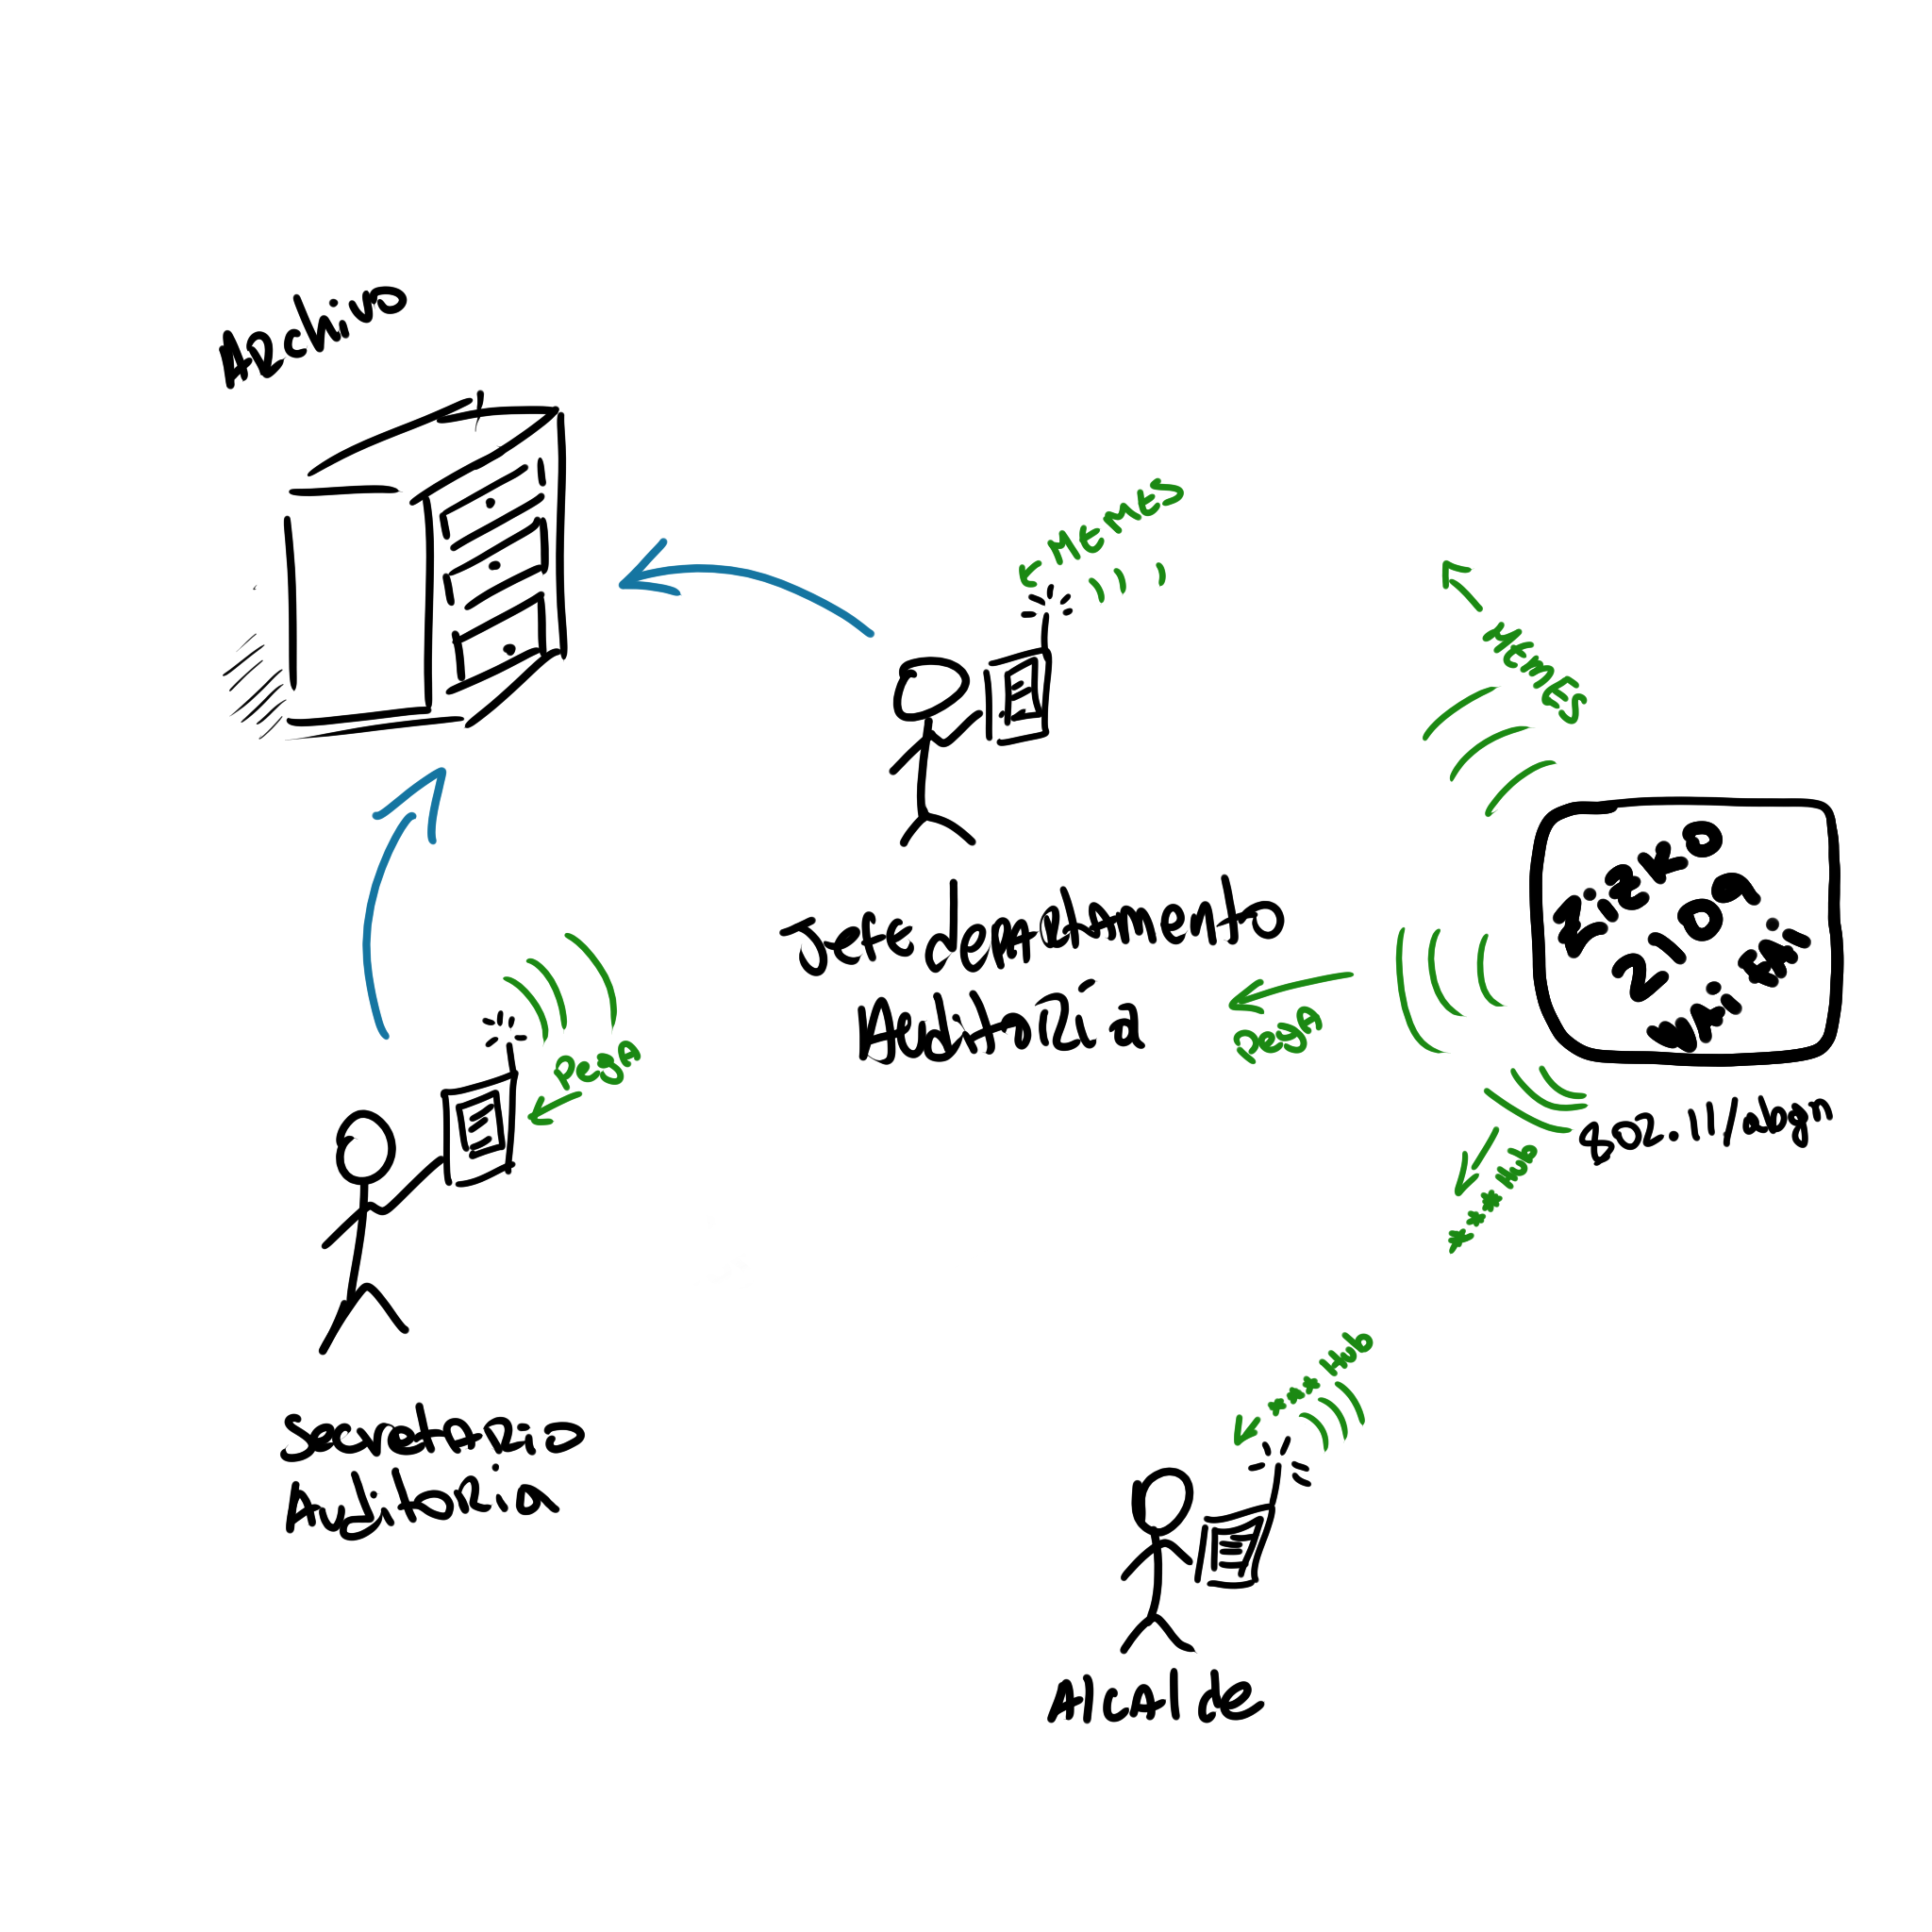
\includegraphics[width=.7\textwidth]{./auditoria/10.png}\\
	\end{figure}
\end{frame}

\begin{frame}[c,fragile]
	\frametitle{Estructura de los activos - Simplificado}
	\begin{figure}[H]
		\centering
		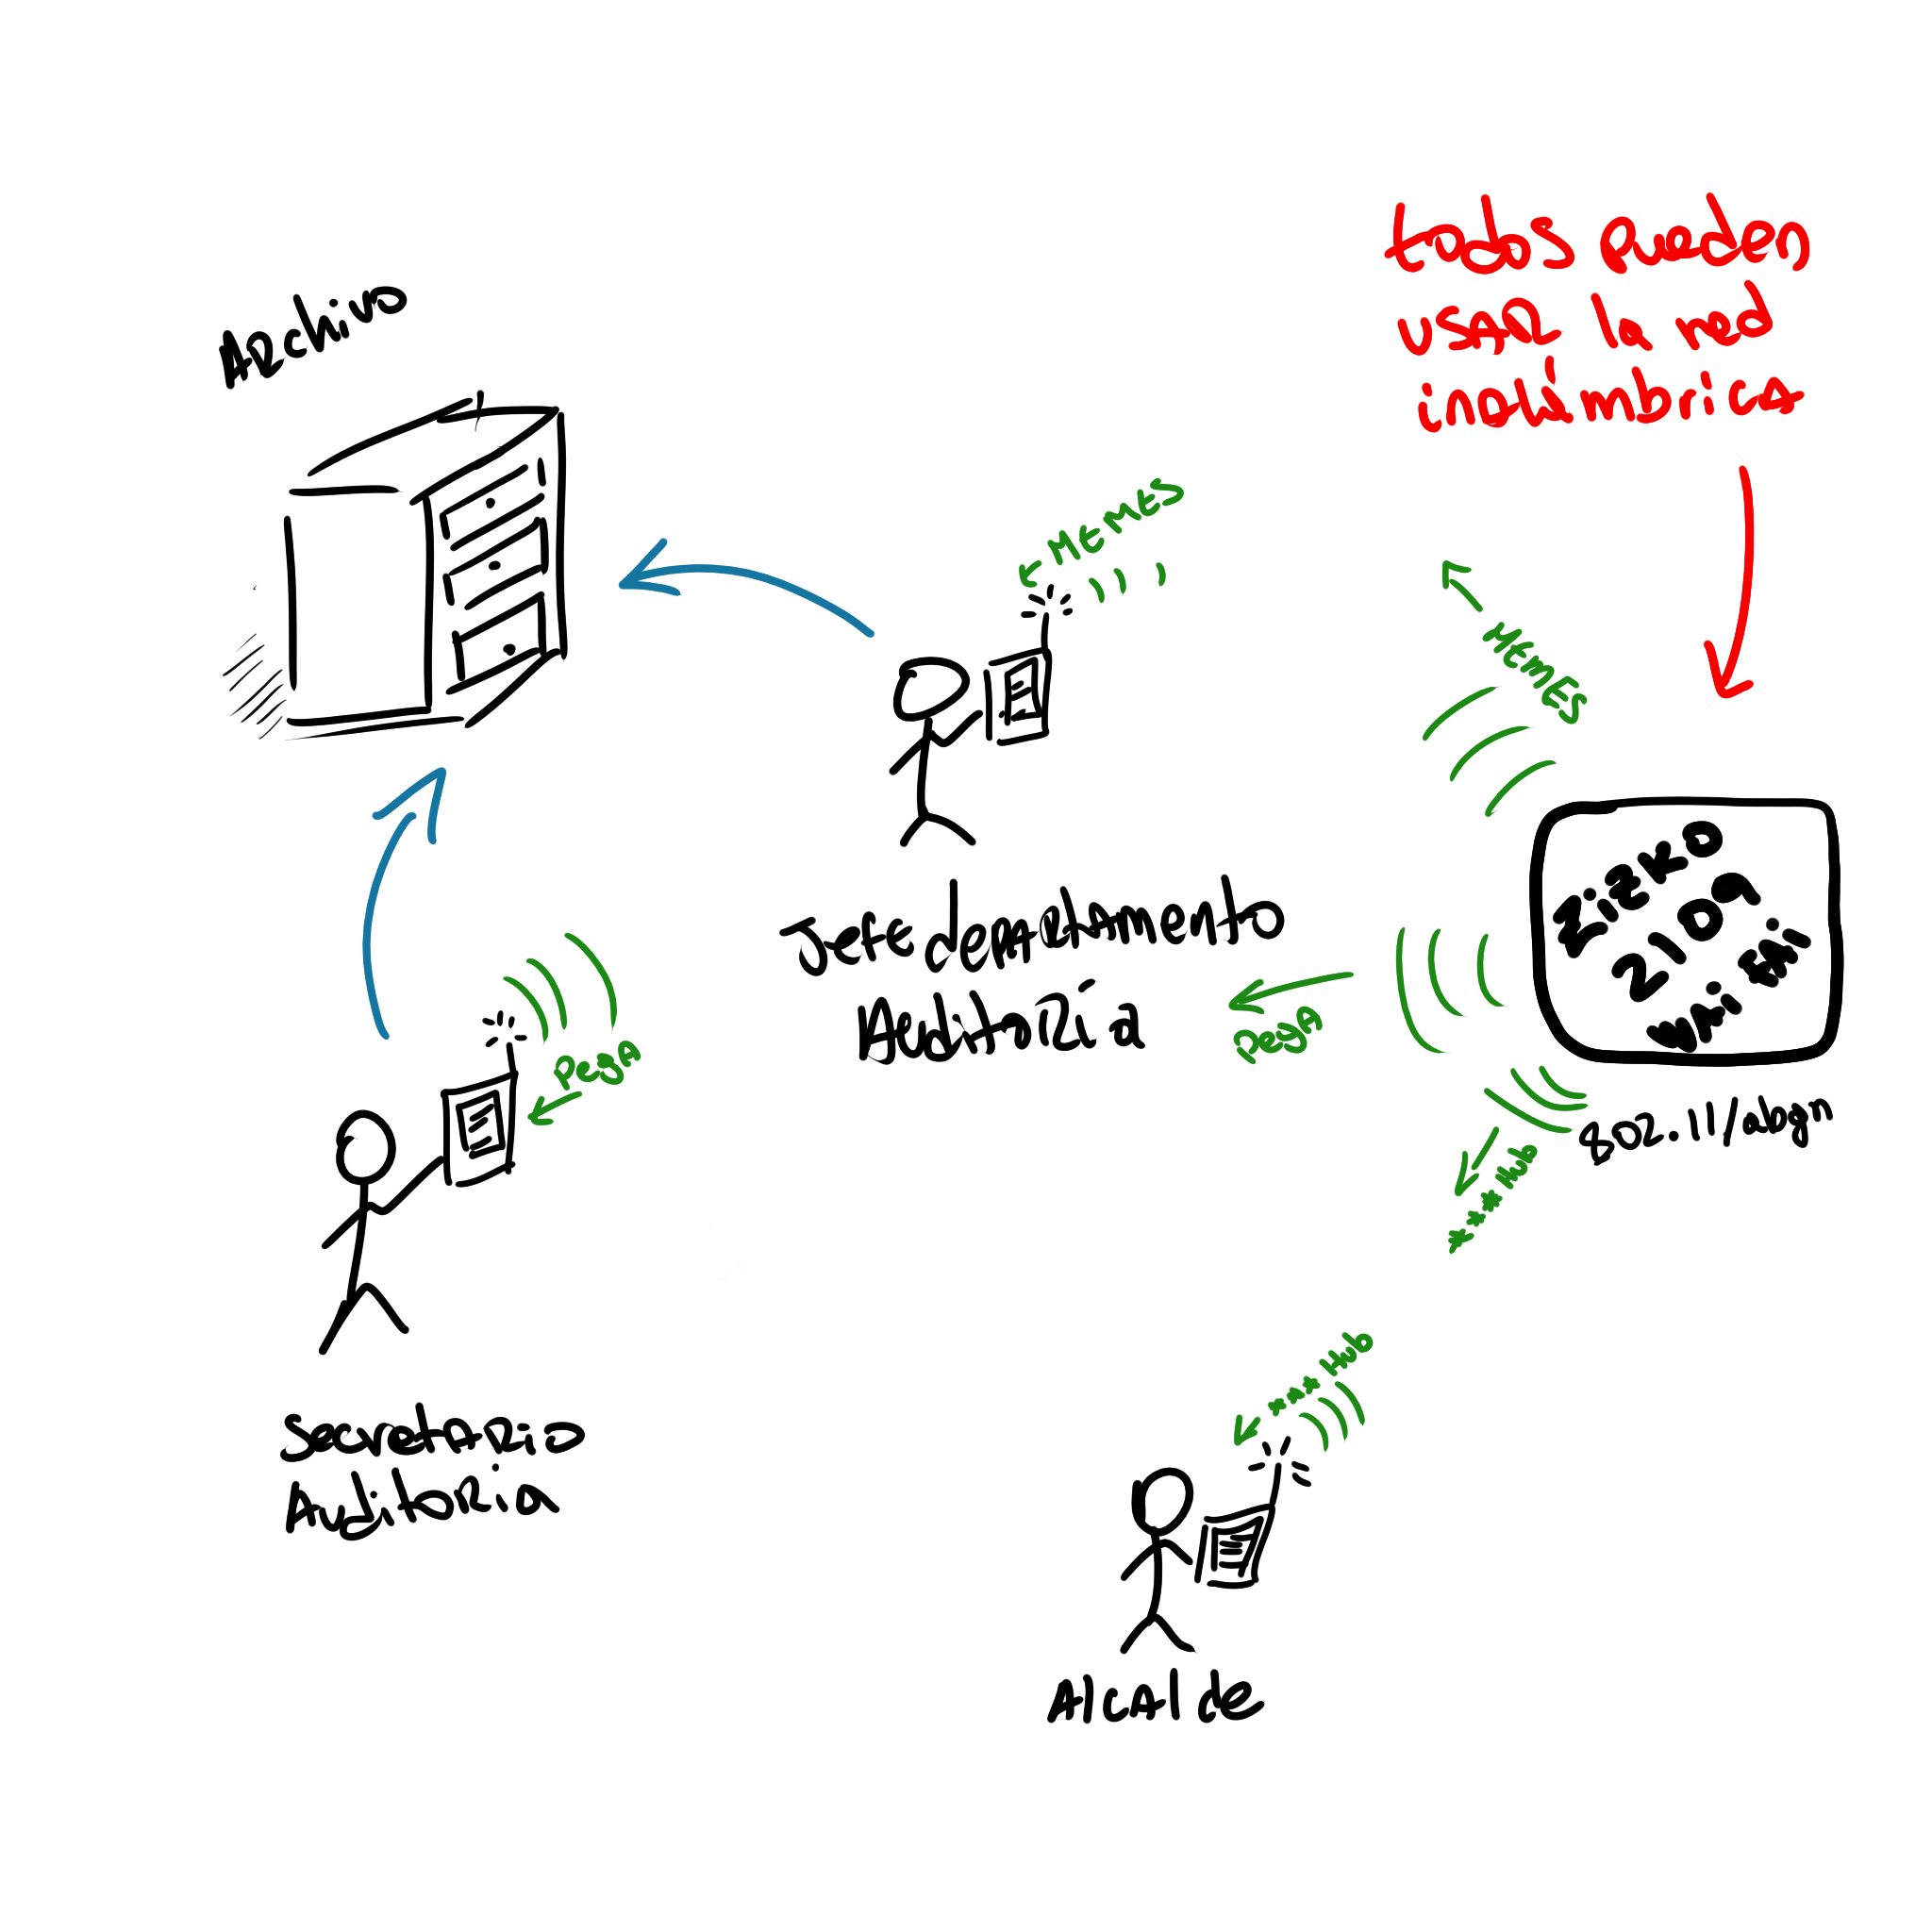
\includegraphics[width=.7\textwidth]{./auditoria/11.png}\\
	\end{figure}
\end{frame}



\section{Contenido del reporte}
\begin{frame}[c,fragile]
	\frametitle{Resumen}
	\begin{itemize}
		\item{121 activos listados
			\begin{itemize}
				\item 19 transversales
				\item 4 externos
				\item 98 especìficos
			\end{itemize}
		}
		\item{35 Amenazas
			\item{ Fragmentadas por tipo 
				\begin{itemize}
					\item Riesgos asociados a factores no tecnológicos
					\item Riesgos asociados a procesos municpales
					\item Riesgos asociados a control del personal
					\item Riesgos asociados de índole técnica
					\item Riesgos generales asociados a ingenería social
				\end{itemize}
			}
		}
	\end{itemize}
\end{frame}

\begin{frame}[c,fragile]
	\frametitle{Evaluación}
		\begin{itemize}
			\item 5 con impacto catastrófico
			\item 8 con impacto alto
			\item 6 con criticidad máxima
			\item 8 con criticidad alta
			\item 6 con probabilidad de ocurrencia sobre 60\%
		\end{itemize}
\end{frame}

\begin{frame}[c,fragile]
	\frametitle{Riesgos notables pt.1}
	\begin{itemize}
		\begin{itemize}
			\item Desastres lógicos.
			\item Divulgación y copiado de informacion.
			\item Candados de seguridad.
			\item Falta de documentación e implantación de políticas para envío de correos masivos.
			\item Falta de punto de contacto.
			\item Roles no definidos.
			\item Falta de monitoreo.
			\item Obtención y/o renovación de permisos de circulación sin ingreso o acreditación física y online de datos sobre propietario, placa patente única, seguro obligatorio, revisión técnica y/o multas impagas.
			\item Recepción de pagos con cálculos de intereses y multas fuera de período.
			\item Quiebre autenticación de llave seguridad.
		\end{itemize}
	\end{itemize}
\end{frame}

\begin{frame}[c,fragile]
	\frametitle{Riesgos notables pt.2}
	\begin{itemize}
		\begin{itemize}
			\item Analfabetismo digital.
			\item Transaccion rota.
			\item Falta de encriptado.
			\item Residuos de información.
			\item Denegación de servicio.
			\item Phishing.
			\item Desastres naturales.
			\item Desastres de origen humano.
			\item Perdida o robo.
			\item Inexistencia de respaldos digitales.
			\item Inexistencia de respaldos físicos.
			\item Falta de protocolo de borrado de información.
			\item Copia de llaves.
			\item No interoperabilidad con estándar de norma técnica para los Órganos de la Administración del Estado.
		\end{itemize}
	\end{itemize}
\end{frame}


\begin{frame}[c,fragile]
	\frametitle{Consideraciones de las políticas emitidas}
	\begin{itemize}
		\item Base para el uso correcto de recursos digitales.
		\item No considera factores culturales.
		\item Intencionalmente no establece dependencias respecto de los departamentos de informática.
		\item Pensada en el uso de recursos digitales, como el acceso a intener, acceso remoto e instrucciones generales para el manejo de incidentes.
	\end{itemize}
\end{frame}


% Creates title page of slide show using above information
\begin{frame}
	\titlepage
  \end{frame}
\end{document}
